\documentclass[]{article}
\usepackage{lmodern}
\usepackage{amssymb,amsmath}
\usepackage{ifxetex,ifluatex}
\usepackage{fixltx2e} % provides \textsubscript
\ifnum 0\ifxetex 1\fi\ifluatex 1\fi=0 % if pdftex
  \usepackage[T1]{fontenc}
  \usepackage[utf8]{inputenc}
\else % if luatex or xelatex
  \ifxetex
    \usepackage{mathspec}
  \else
    \usepackage{fontspec}
  \fi
  \defaultfontfeatures{Ligatures=TeX,Scale=MatchLowercase}
\fi
% use upquote if available, for straight quotes in verbatim environments
\IfFileExists{upquote.sty}{\usepackage{upquote}}{}
% use microtype if available
\IfFileExists{microtype.sty}{%
\usepackage{microtype}
\UseMicrotypeSet[protrusion]{basicmath} % disable protrusion for tt fonts
}{}
\usepackage[margin=1in]{geometry}
\usepackage{hyperref}
\hypersetup{unicode=true,
            pdftitle={Citations Analysis of Letter Signers},
            pdfauthor={Joshua Paik and Igor Rivin},
            pdfborder={0 0 0},
            breaklinks=true}
\urlstyle{same}  % don't use monospace font for urls
\usepackage{color}
\usepackage{fancyvrb}
\newcommand{\VerbBar}{|}
\newcommand{\VERB}{\Verb[commandchars=\\\{\}]}
\DefineVerbatimEnvironment{Highlighting}{Verbatim}{commandchars=\\\{\}}
% Add ',fontsize=\small' for more characters per line
\usepackage{framed}
\definecolor{shadecolor}{RGB}{248,248,248}
\newenvironment{Shaded}{\begin{snugshade}}{\end{snugshade}}
\newcommand{\AlertTok}[1]{\textcolor[rgb]{0.94,0.16,0.16}{#1}}
\newcommand{\AnnotationTok}[1]{\textcolor[rgb]{0.56,0.35,0.01}{\textbf{\textit{#1}}}}
\newcommand{\AttributeTok}[1]{\textcolor[rgb]{0.77,0.63,0.00}{#1}}
\newcommand{\BaseNTok}[1]{\textcolor[rgb]{0.00,0.00,0.81}{#1}}
\newcommand{\BuiltInTok}[1]{#1}
\newcommand{\CharTok}[1]{\textcolor[rgb]{0.31,0.60,0.02}{#1}}
\newcommand{\CommentTok}[1]{\textcolor[rgb]{0.56,0.35,0.01}{\textit{#1}}}
\newcommand{\CommentVarTok}[1]{\textcolor[rgb]{0.56,0.35,0.01}{\textbf{\textit{#1}}}}
\newcommand{\ConstantTok}[1]{\textcolor[rgb]{0.00,0.00,0.00}{#1}}
\newcommand{\ControlFlowTok}[1]{\textcolor[rgb]{0.13,0.29,0.53}{\textbf{#1}}}
\newcommand{\DataTypeTok}[1]{\textcolor[rgb]{0.13,0.29,0.53}{#1}}
\newcommand{\DecValTok}[1]{\textcolor[rgb]{0.00,0.00,0.81}{#1}}
\newcommand{\DocumentationTok}[1]{\textcolor[rgb]{0.56,0.35,0.01}{\textbf{\textit{#1}}}}
\newcommand{\ErrorTok}[1]{\textcolor[rgb]{0.64,0.00,0.00}{\textbf{#1}}}
\newcommand{\ExtensionTok}[1]{#1}
\newcommand{\FloatTok}[1]{\textcolor[rgb]{0.00,0.00,0.81}{#1}}
\newcommand{\FunctionTok}[1]{\textcolor[rgb]{0.00,0.00,0.00}{#1}}
\newcommand{\ImportTok}[1]{#1}
\newcommand{\InformationTok}[1]{\textcolor[rgb]{0.56,0.35,0.01}{\textbf{\textit{#1}}}}
\newcommand{\KeywordTok}[1]{\textcolor[rgb]{0.13,0.29,0.53}{\textbf{#1}}}
\newcommand{\NormalTok}[1]{#1}
\newcommand{\OperatorTok}[1]{\textcolor[rgb]{0.81,0.36,0.00}{\textbf{#1}}}
\newcommand{\OtherTok}[1]{\textcolor[rgb]{0.56,0.35,0.01}{#1}}
\newcommand{\PreprocessorTok}[1]{\textcolor[rgb]{0.56,0.35,0.01}{\textit{#1}}}
\newcommand{\RegionMarkerTok}[1]{#1}
\newcommand{\SpecialCharTok}[1]{\textcolor[rgb]{0.00,0.00,0.00}{#1}}
\newcommand{\SpecialStringTok}[1]{\textcolor[rgb]{0.31,0.60,0.02}{#1}}
\newcommand{\StringTok}[1]{\textcolor[rgb]{0.31,0.60,0.02}{#1}}
\newcommand{\VariableTok}[1]{\textcolor[rgb]{0.00,0.00,0.00}{#1}}
\newcommand{\VerbatimStringTok}[1]{\textcolor[rgb]{0.31,0.60,0.02}{#1}}
\newcommand{\WarningTok}[1]{\textcolor[rgb]{0.56,0.35,0.01}{\textbf{\textit{#1}}}}
\usepackage{graphicx,grffile}
\makeatletter
\def\maxwidth{\ifdim\Gin@nat@width>\linewidth\linewidth\else\Gin@nat@width\fi}
\def\maxheight{\ifdim\Gin@nat@height>\textheight\textheight\else\Gin@nat@height\fi}
\makeatother
% Scale images if necessary, so that they will not overflow the page
% margins by default, and it is still possible to overwrite the defaults
% using explicit options in \includegraphics[width, height, ...]{}
\setkeys{Gin}{width=\maxwidth,height=\maxheight,keepaspectratio}
\IfFileExists{parskip.sty}{%
\usepackage{parskip}
}{% else
\setlength{\parindent}{0pt}
\setlength{\parskip}{6pt plus 2pt minus 1pt}
}
\setlength{\emergencystretch}{3em}  % prevent overfull lines
\providecommand{\tightlist}{%
  \setlength{\itemsep}{0pt}\setlength{\parskip}{0pt}}
\setcounter{secnumdepth}{0}
% Redefines (sub)paragraphs to behave more like sections
\ifx\paragraph\undefined\else
\let\oldparagraph\paragraph
\renewcommand{\paragraph}[1]{\oldparagraph{#1}\mbox{}}
\fi
\ifx\subparagraph\undefined\else
\let\oldsubparagraph\subparagraph
\renewcommand{\subparagraph}[1]{\oldsubparagraph{#1}\mbox{}}
\fi

%%% Use protect on footnotes to avoid problems with footnotes in titles
\let\rmarkdownfootnote\footnote%
\def\footnote{\protect\rmarkdownfootnote}

%%% Change title format to be more compact
\usepackage{titling}

% Create subtitle command for use in maketitle
\providecommand{\subtitle}[1]{
  \posttitle{
    \begin{center}\large#1\end{center}
    }
}

\setlength{\droptitle}{-2em}

  \title{Citations Analysis of Letter Signers}
    \pretitle{\vspace{\droptitle}\centering\huge}
  \posttitle{\par}
    \author{Joshua Paik and Igor Rivin}
    \preauthor{\centering\large\emph}
  \postauthor{\par}
      \predate{\centering\large\emph}
  \postdate{\par}
    \date{12/31/2019}


\begin{document}
\maketitle

{
\setcounter{tocdepth}{2}
\tableofcontents
}
\hypertarget{introduction}{%
\subsection{Introduction}\label{introduction}}

In November 2019, Abigail Thompson, chair of Mathematics at UC Davis and
Vice President of the American Mathematical Society, published an essay
{[}\protect\hyperlink{Bibliography}{1}{]} in the Notices of the AMS that
criticized the usage of Mandatory Diversity Statements when hiring
mathematics faculty. She described Diversity Statements as a ``political
test'' and compared it to McCarthyism.

In December 2019, a multitude of responses to Thompson's Letter were
published in Notices {[}\protect\hyperlink{Bibliography}{2}{]},
accumulating hundreds of signatures. One letter, titled ``The math
community values a commitment to diversity,'' ``strongly (disagreed)
with the sentiments and arguments in Dr.~Thompson's editorial,'' and
hoped ``that the AMS will reconsider the way that it uses its power and
position in the mathematics communities in these kinds of discussions.''
Another letter, titled ``Letter to the Editor,'' spoke of ``grave
concerns about recent attempts to intimidate a voice within our
mathematical community.'' In this letter, they reference a blog post
which encouraged faculty to ``advise grad-school-bound undergraduate
students -- especially students who are minoritized along some axis --
not to apply to UC Davis.'' {[}\protect\hyperlink{Bibliography}{3}{]} A
final letter, titled ``Letter to the Notices of the AMS,'' criticized
the usage of mandatory diversity statements, but affirmed the importance
of diversity in mathematics.

For the purpose of this exploration, Letter A will refer to the letter
titled ``The math community values a commitment to diversity,'' Letter B
will refer to the one titled ``Letter to the Editor,'' and Letter C will
refer to the one titled ``Letter to the Notices of the AMS.''

We will analyze the age (relative to PhD year) and gender of letter
signers. We will also analyze the number of MathSciNet citations and
citations per year of letter signers in this study. We will also analyze
the number of Google Scholar citations, citation per year and h-index of
letter signers. We prefer MathSciNet because only published mathematics
are in MathSciNet, and is hence a higher quality data source when
comparing mathematicians. We also assess the distributions of MathSciNet
and Google Scholar citations.

It should be noted and emphasized that citations and h-indices do not
impose a total order on the quality of a mathematician. Stephen Smale
has less citations than Terrence Tao, but it would be a challenging and
an unfruitful exercise to distinguish who is in fact the better
mathematician. However, citations generally reflect the mathematics
communities opinion of a person, and is the only empirical metric of
assessing this.

\hypertarget{data-collection}{%
\subsection{Data Collection}\label{data-collection}}

Data was collected on December 16-18, 2019 from Google Scholar and the
Mathematics Genealogy Project. After a list of names and affiliations
were scraped from the AMS response letters, signers were searched on
Google Scholar and their citation numbers and h-index were collected.
This was done using the scholarly API and manual
checks.{[}\protect\hyperlink{Bibliography}{4}{]}
{[}\protect\hyperlink{Bibliography}{5}{]} Then the
math-genealogy-scraper was used to calculate PhD years and errors
(duplicate names) were also corrected manually.
{[}\protect\hyperlink{Bibliography}{6}{]}
{[}\protect\hyperlink{Bibliography}{7}{]}. MathSciNet entries were
collected manually. Finally, the data was merged with the QSIDE dataset
released on December 28th {[}\protect\hyperlink{Bibliography}{8}{]}.

\hypertarget{summary-statistics}{%
\subsection{Summary Statistics}\label{summary-statistics}}

\begin{verbatim}
##        X1             name           affiliation          citations    
##  Min.   :   0.0   Length:1435        Length:1435        Min.   :    1  
##  1st Qu.: 358.5   Class :character   Class :character   1st Qu.:  158  
##  Median : 717.0   Mode  :character   Mode  :character   Median :  831  
##  Mean   : 717.0                                         Mean   : 2796  
##  3rd Qu.:1075.5                                         3rd Qu.: 2840  
##  Max.   :1434.0                                         Max.   :71530  
##                                                         NA's   :920    
##      hindex            year       lettergroup        gender   
##  Min.   :  1.00   Min.   :1957   A and B:  6   man      :969  
##  1st Qu.:  6.00   1st Qu.:1984   A Only :615   nonbinary:  1  
##  Median : 15.00   Median :1999   B and C: 74   woman    :452  
##  Mean   : 18.45   Mean   :1996   B Only :600   NA's     : 13  
##  3rd Qu.: 26.00   3rd Qu.:2009   C Only :134                  
##  Max.   :106.00   Max.   :2019   NA's   :  6                  
##  NA's   :922      NA's   :553                                 
##         highered           institution    research             country    
##  highered   :1361   domesticother:379   lessri:487   israel        :  46  
##  nothighered:  41   domesticr1   :673   moreri:878   canada        :  37  
##  NA's       :  33   domesticr2   :108   NA's  : 70   united kingdom:  21  
##                     international:205                germany       :  14  
##                     NA's         : 70                france        :  13  
##                                                      (Other)       :  49  
##                                                      NA's          :1255  
##         role           security      field        simplefield  
##  professor:635   lesssecure:425   comp  :  16   mathed  :  33  
##  associate:202   moresecure:902   math  :1216   mathstat:1228  
##  assistant:192   NA's      :108   mathed:  33   other   :  90  
##  grad     :119                    other :  74   NA's    :  84  
##  ntt      : 97                    stat  :  12                  
##  (Other)  : 83                    NA's  :  84                  
##  NA's     :107                                                 
##   fellows            amscit           Fields               age       
##  Mode :logical   Min.   :    0.0   Length:1435        Min.   : 1.00  
##  FALSE:1223      1st Qu.:  447.5   Class :character   1st Qu.:11.00  
##  TRUE :206       Median : 1006.0   Mode  :character   Median :21.00  
##  NA's :6         Mean   : 1650.5                      Mean   :23.87  
##                  3rd Qu.: 1813.5                      3rd Qu.:36.00  
##                  Max.   :15430.0                      Max.   :63.00  
##                  NA's   :1131                         NA's   :553    
##    citperyear       amscitperyear   
##  Min.   :   0.118   Min.   :  0.00  
##  1st Qu.:  18.688   1st Qu.: 15.96  
##  Median :  48.062   Median : 27.55  
##  Mean   : 113.541   Mean   : 44.95  
##  3rd Qu.: 111.271   3rd Qu.: 52.19  
##  Max.   :3223.524   Max.   :642.92  
##  NA's   :1056       NA's   :1188
\end{verbatim}

\hypertarget{exploratory-data-analysis}{%
\section{Exploratory Data Analysis}\label{exploratory-data-analysis}}

\hypertarget{nan-visualization}{%
\subsection{NaN Visualization}\label{nan-visualization}}

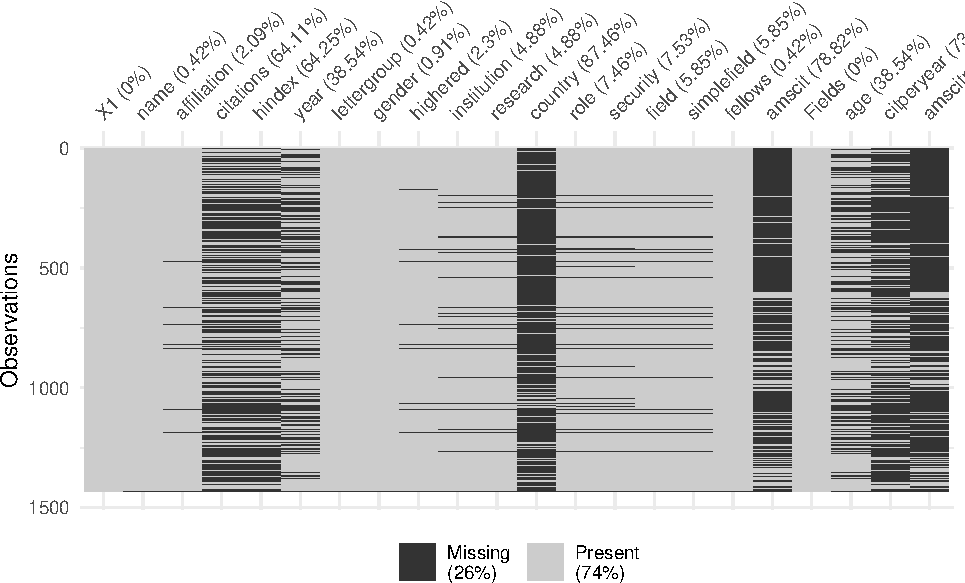
\includegraphics{final_files/figure-latex/unnamed-chunk-3-1.pdf}

The citations and h-index column refers to citations and h-indices
pulled from Google Scholar. The amscit column refers to citations pulled
from Math Sci Net. The year column refers to PhD years scraped from the
Mathematics Genealogy Project. The age column was induced by subtracting
2020 from PhD years. The citperyear and amscitper year columns were
induced by dividing citations by age. The fellows column refer to
individuals who are fellows of the AMS.

64.11\% of the Google Scholar citations is NaN, and 75.47\% of the
mathscinet citations is NaN. While this is not optimal, a quick sample
size calculation shows that one needs 303 samples or 21\% of the data to
produce statistics at a 95\% confidence level and a 5\% confidence
interval.

\hypertarget{distribution-of-google-scholar-citations}{%
\subsection{Distribution of Google Scholar
Citations}\label{distribution-of-google-scholar-citations}}

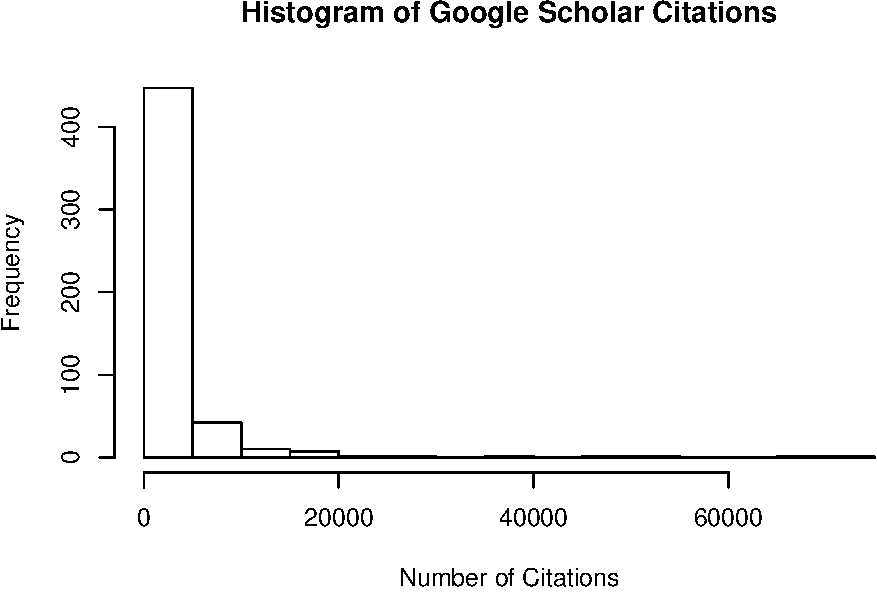
\includegraphics{final_files/figure-latex/unnamed-chunk-4-1.pdf}

The data is heavily left skewed. This is usually handled either by
transforming the data with a natural logarithm, or by square rooting.
Applying a logarithm is a more appropiate transformation to assess
normality, and a square root is more appropriate to assess
exponentiality. We try both.

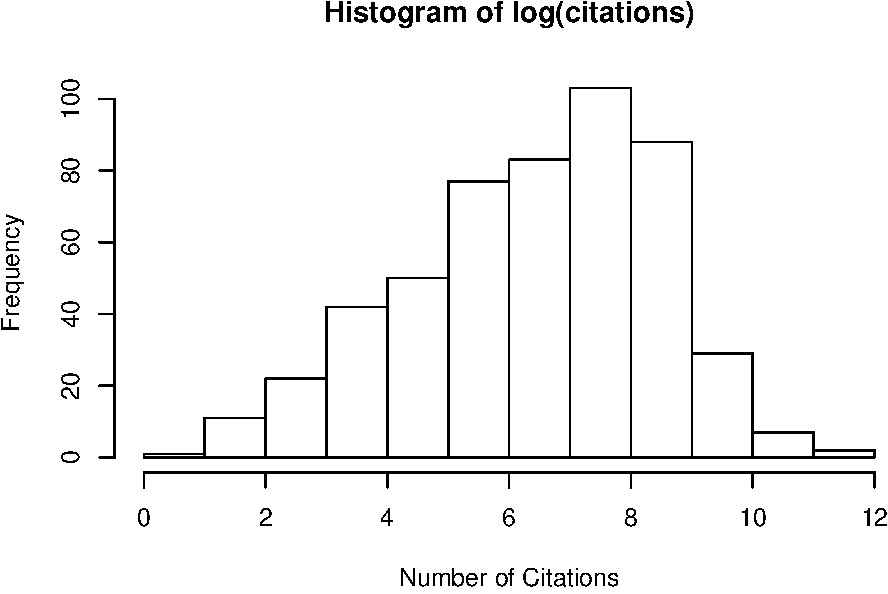
\includegraphics{final_files/figure-latex/unnamed-chunk-5-1.pdf}

This data is now right skewed.

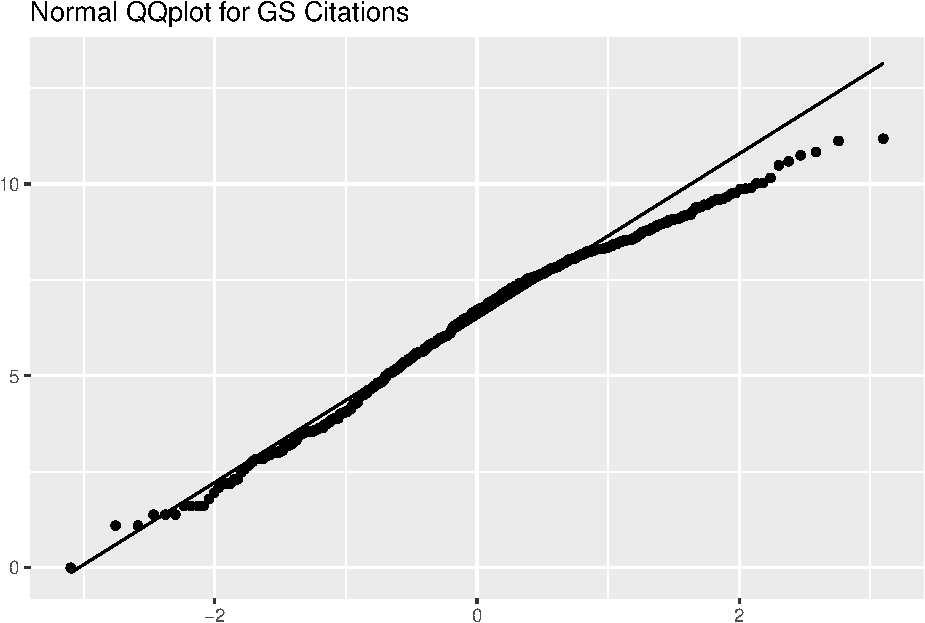
\includegraphics{final_files/figure-latex/unnamed-chunk-6-1.pdf}

The data is heavy towards the center, and the tails are sparsely
populated. Hence the data is unlikely to be normally distributed.

If we construct a qq-plot with a fitted exponential curve, we find that
there is divergence in the tails.

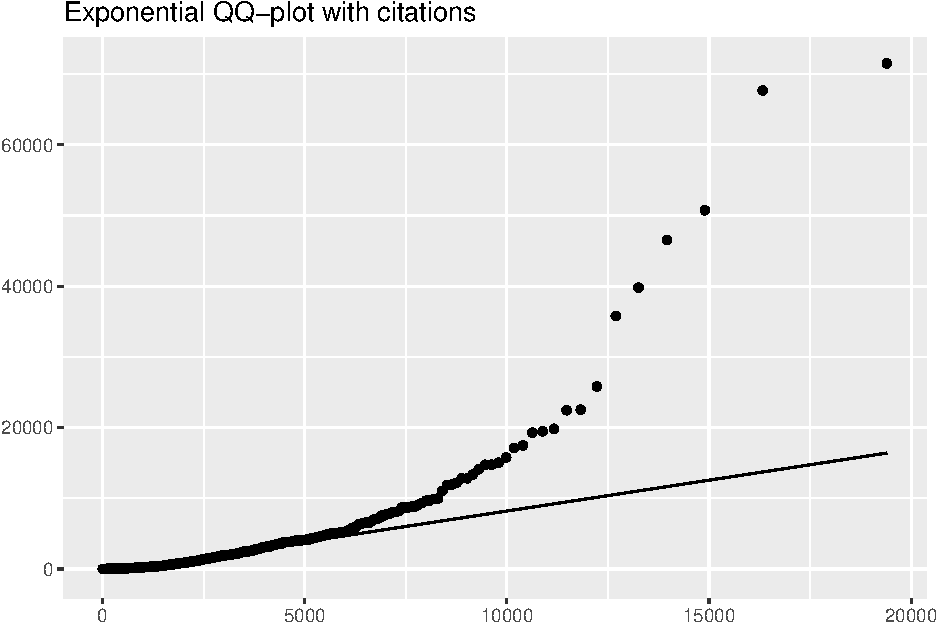
\includegraphics{final_files/figure-latex/unnamed-chunk-7-1.pdf}

We now apply a square root.

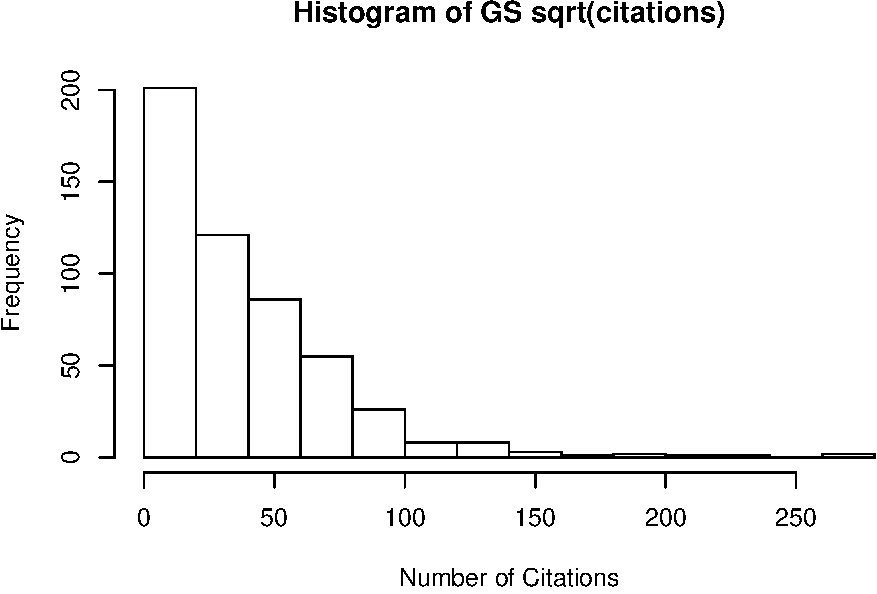
\includegraphics{final_files/figure-latex/unnamed-chunk-8-1.pdf}

This looks like an exponential distribution.

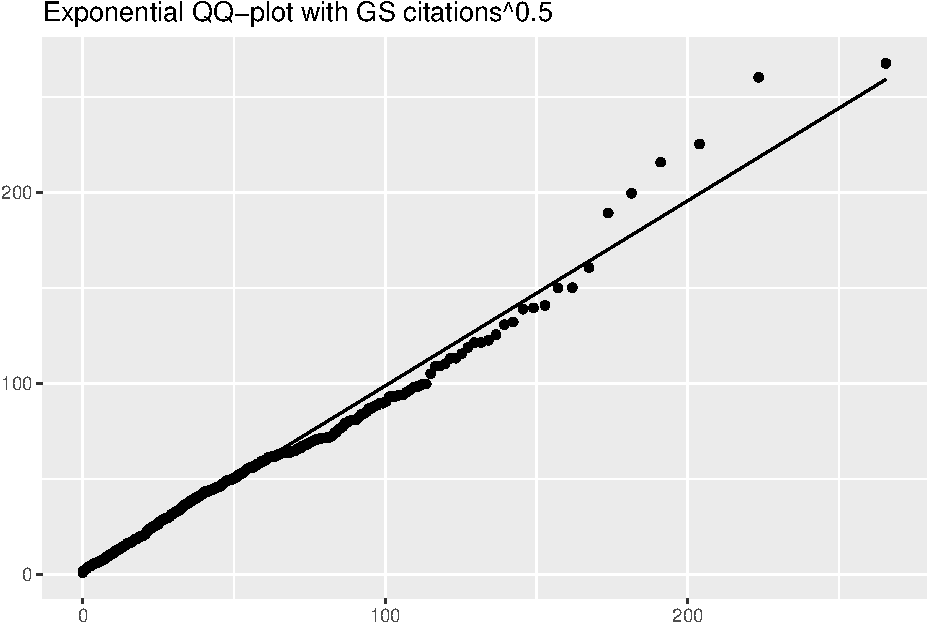
\includegraphics{final_files/figure-latex/unnamed-chunk-9-1.pdf}

An exponential distribution seems to fit the data better, post square
rooting. Some fine tuning shows that raising the data to 0.46 produces
the closest approximation to an exponential distribution.

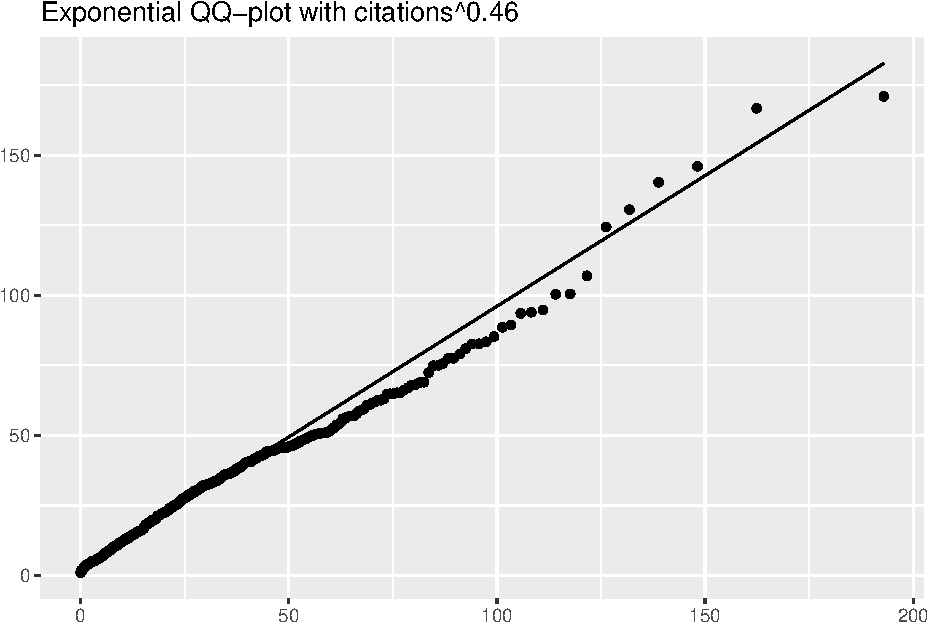
\includegraphics{final_files/figure-latex/unnamed-chunk-10-1.pdf}

\hypertarget{distribution-of-mathscinet-citations}{%
\subsection{Distribution of MathSciNet
citations}\label{distribution-of-mathscinet-citations}}

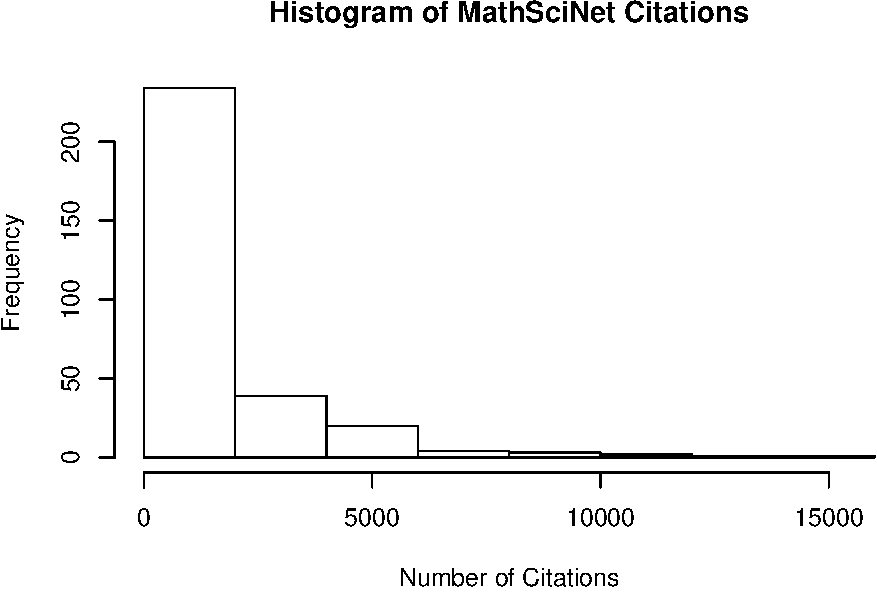
\includegraphics{final_files/figure-latex/unnamed-chunk-11-1.pdf}

The data is again left skewed. Fitting an exponential distribution to
this data, we see that there is divergence in the tails.

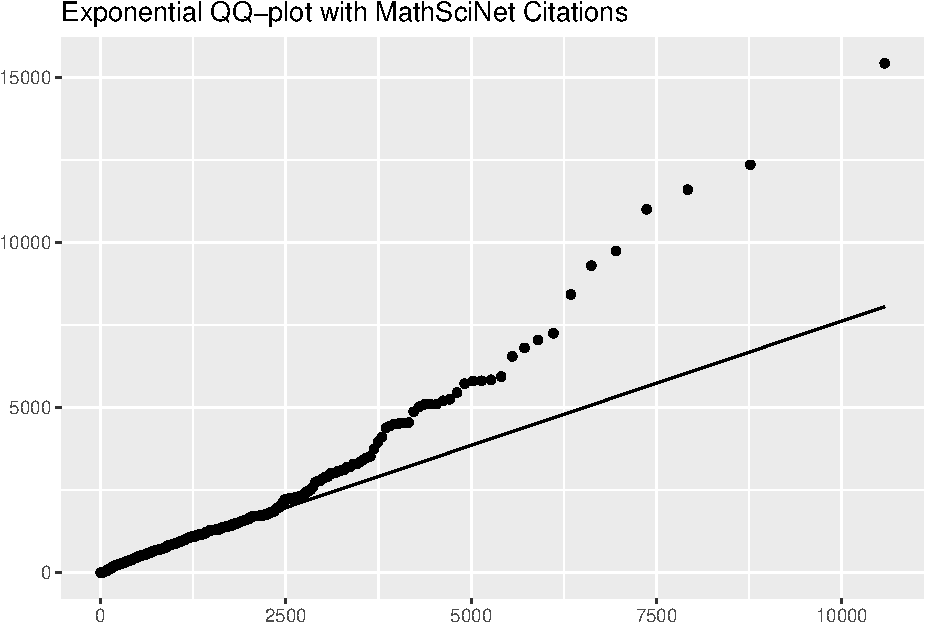
\includegraphics{final_files/figure-latex/unnamed-chunk-12-1.pdf}

We now apply a square root.

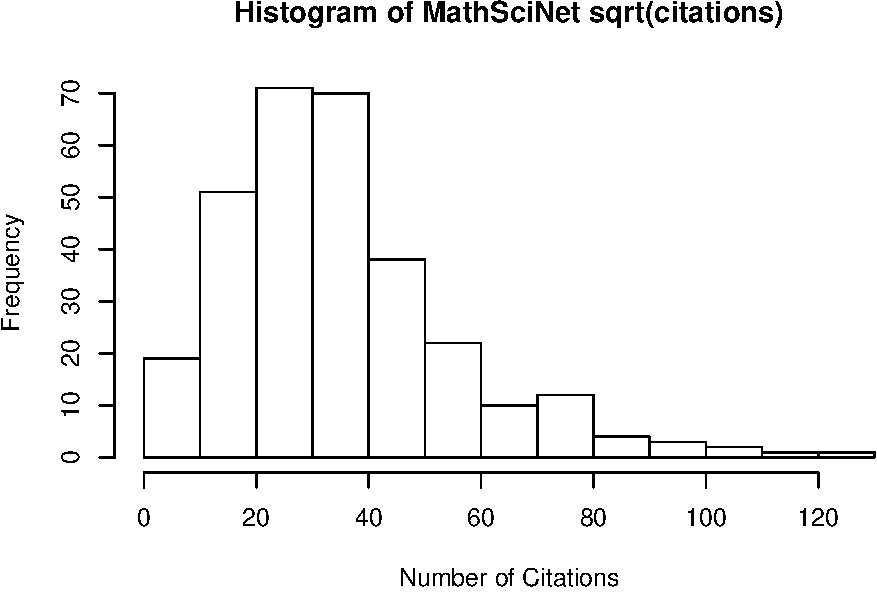
\includegraphics{final_files/figure-latex/unnamed-chunk-13-1.pdf}

The data again looks approximately exponentially distributed, except for
the data on the right. This is due to the presence of academics with
zero citations.

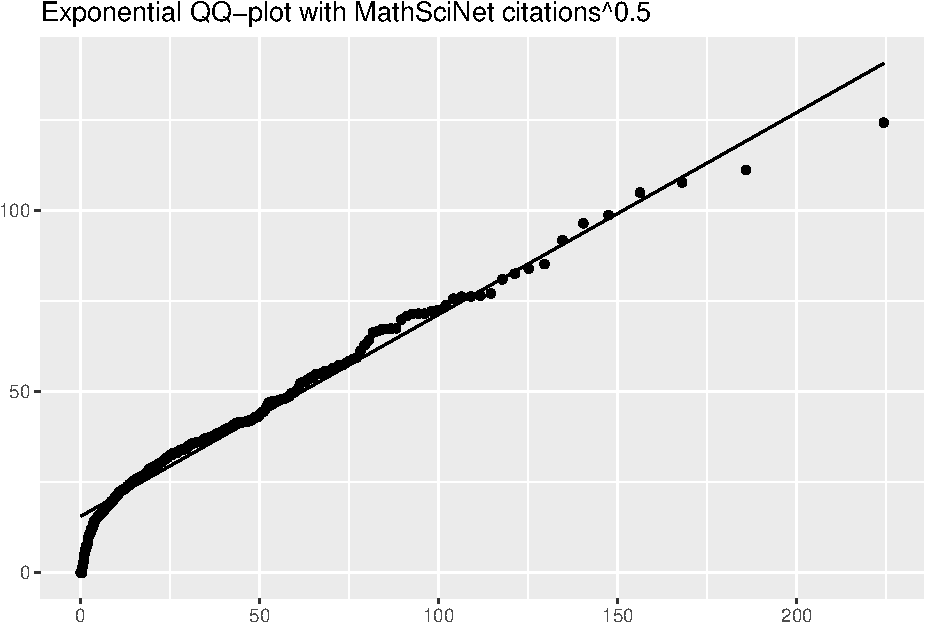
\includegraphics{final_files/figure-latex/unnamed-chunk-14-1.pdf}

The divergence in the left tail is caused by a number of mathematicians
with zero citations. Some fine tuning shows that raising the data to
0.54 produces the closest approximation to an exponential distribution.

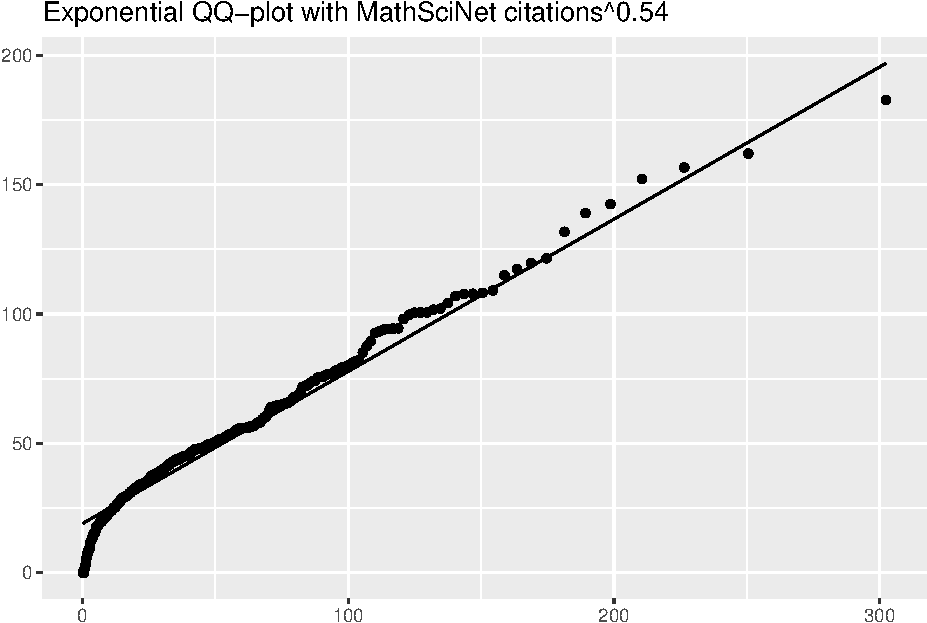
\includegraphics{final_files/figure-latex/unnamed-chunk-15-1.pdf}

If we check if the data is Normally distributed, we see again that there
is sparsity in the tails. Hence it is unlikely that the data is log
normal.
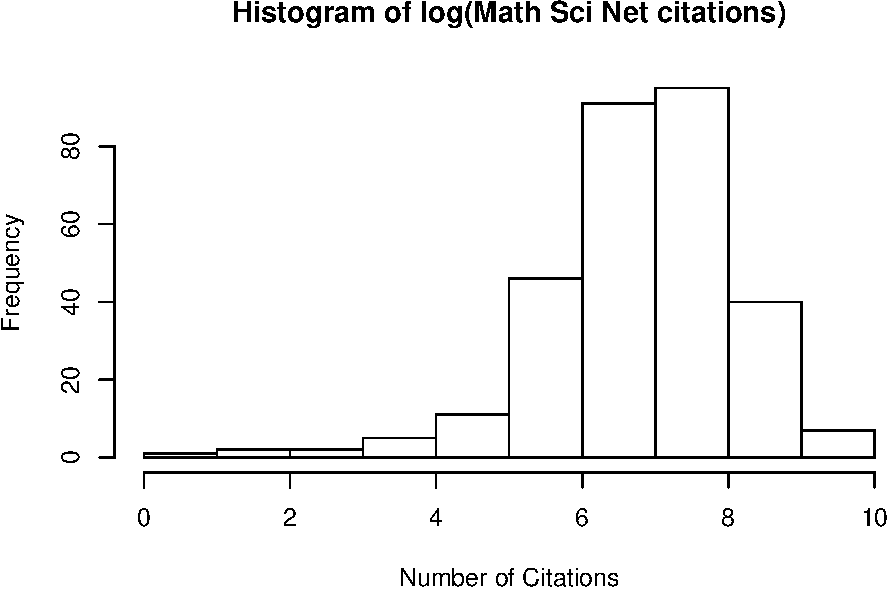
\includegraphics{final_files/figure-latex/unnamed-chunk-16-1.pdf}

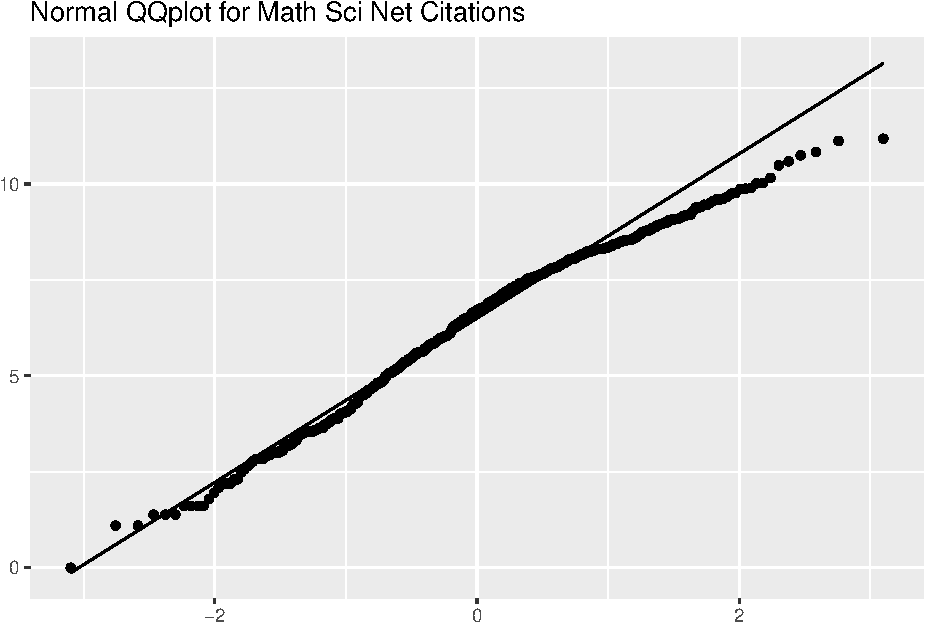
\includegraphics{final_files/figure-latex/unnamed-chunk-17-1.pdf}

So the MathSciNet data and GS data, when appropriately transformed,
appear to be approximately Exponentially distributed.

\hypertarget{permutation-tests}{%
\subsection{Permutation Tests}\label{permutation-tests}}

A permutation test is a nonparametric way of assessing the difference in
mean between two populations. We are interested in whether an observed
difference in mean is due to chance, and we can assess this in the
following way.

\begin{enumerate}
\def\labelenumi{\arabic{enumi}.}
\setcounter{enumi}{-1}
\tightlist
\item
  Record the true difference in mean (\(d\mu\)).
\item
  \(H_0: d\mu = 0, H_1: d\mu < 0\)
\item
  Sample without replacement 1/2 of the combined data set (X) and what
  is left (Y)
\item
  Take the mean of X and Y and record the difference
\item
  Repeat 10,000 times and plot the histogram
\item
  Record the number of points (m) in the induced distribution that is
  more extreme than or equal to the observed \(d\mu\). The probability
  m/10,000 is the probability that what was observed was due to chance.
\end{enumerate}

Here is the function we will use to do this.

\begin{Shaded}
\begin{Highlighting}[]
\CommentTok{# input data and the number of permutations}
\NormalTok{meanPermutation <-}\StringTok{ }\ControlFlowTok{function}\NormalTok{(Data, n)\{}
\NormalTok{  output <-}\StringTok{ }\KeywordTok{matrix}\NormalTok{(}\OtherTok{NA}\NormalTok{, }\DataTypeTok{ncol =} \DecValTok{1}\NormalTok{, }\DataTypeTok{nrow =}\NormalTok{ n)}
  \ControlFlowTok{for}\NormalTok{(i }\ControlFlowTok{in} \DecValTok{1}\OperatorTok{:}\NormalTok{n)\{}
    \CommentTok{#sample 1/2 of the data}
\NormalTok{    X_index <-}\StringTok{ }\KeywordTok{sample}\NormalTok{(}\DecValTok{1}\OperatorTok{:}\KeywordTok{length}\NormalTok{(Data), }\KeywordTok{floor}\NormalTok{(}\FloatTok{0.5} \OperatorTok{*}\StringTok{ }\KeywordTok{length}\NormalTok{(Data)))}
\NormalTok{    Y_index <-}\StringTok{ }\KeywordTok{setdiff}\NormalTok{(}\DecValTok{1}\OperatorTok{:}\KeywordTok{length}\NormalTok{(Data), X_index)}
\NormalTok{    X <-}\StringTok{ }\NormalTok{Data[X_index]}
\NormalTok{    Y <-}\StringTok{ }\NormalTok{Data[Y_index]}
    \CommentTok{#calculate the difference}
\NormalTok{    diff <-}\StringTok{ }\KeywordTok{mean}\NormalTok{(X)}\OperatorTok{-}\KeywordTok{mean}\NormalTok{(Y)}
    \CommentTok{#store}
\NormalTok{    output[i, ] <-}\StringTok{ }\NormalTok{diff}
\NormalTok{  \} }
  \KeywordTok{return}\NormalTok{(output)}
\NormalTok{\}}
\end{Highlighting}
\end{Shaded}

The induced probability is similar to p-value, and often produces a
similar p-value to a 2-sample t-test. However, it is not a p-value and
cannot be accurately interpreted using the standard 0.05 significance
benchmark. Instead, probabilities are assessed relatively.

\hypertarget{gender}{%
\subsection{Gender}\label{gender}}

What is the proportion of female professors who signed letters A, B, and
C. According to a 2016 AMS survey
{[}\protect\hyperlink{Bibliography}{9}{]}, 707/4902 = 14.4\% of tenured
professors are women, and including all professionals, 2004/9921 =
20.2\% are women.

We can determine this by using dplyr's filter function.

\begin{Shaded}
\begin{Highlighting}[]
\CommentTok{#search via booleans}
\KeywordTok{table}\NormalTok{(}\KeywordTok{filter}\NormalTok{(df,((lettergroup }\OperatorTok{==}\StringTok{ "A Only"}\OperatorTok{|}\NormalTok{lettergroup }\OperatorTok{==}\StringTok{ "A and B"}\NormalTok{)}\OperatorTok{&}\NormalTok{(role}\OperatorTok{==}\StringTok{"professor"}\NormalTok{)))}\OperatorTok{$}\NormalTok{gender)}
\end{Highlighting}
\end{Shaded}

\begin{verbatim}
## 
##       man nonbinary     woman 
##        79         0        68
\end{verbatim}

On letter A, 68/147 = 46.3\% of professors were women.

\begin{Shaded}
\begin{Highlighting}[]
\KeywordTok{table}\NormalTok{(}\KeywordTok{filter}\NormalTok{(df,((lettergroup }\OperatorTok{==}\StringTok{ "B Only"}\OperatorTok{|}\NormalTok{lettergroup }\OperatorTok{==}\StringTok{ "A and B"}\NormalTok{)}\OperatorTok{&}\NormalTok{(role}\OperatorTok{==}\StringTok{"professor"}\NormalTok{)))}\OperatorTok{$}\NormalTok{gender)}
\end{Highlighting}
\end{Shaded}

\begin{verbatim}
## 
##       man nonbinary     woman 
##       272         0        40
\end{verbatim}

On letter B, 40/312 = 12.8\% of professors were women.

\begin{Shaded}
\begin{Highlighting}[]
\KeywordTok{table}\NormalTok{(}\KeywordTok{filter}\NormalTok{(df,((lettergroup }\OperatorTok{==}\StringTok{ "C Only"}\OperatorTok{|}\NormalTok{lettergroup }\OperatorTok{==}\StringTok{ "B and C"}\NormalTok{)}\OperatorTok{&}\NormalTok{(role}\OperatorTok{==}\StringTok{"professor"}\NormalTok{)))}\OperatorTok{$}\NormalTok{gender)}
\end{Highlighting}
\end{Shaded}

\begin{verbatim}
## 
##       man nonbinary     woman 
##       145         0        37
\end{verbatim}

On letter C, 37/182 = 20.3\% of professors were women.

So while letter A was signed by proportionally more female professors
than the proportion determined by the AMS, letters B and C were
generally reflective of the field, with C over representing the number
of tenured female professors, and B slightly under representing the
number of tenured female professors.

\hypertarget{age}{%
\subsection{Age}\label{age}}

What is the mean age of signers relative to PhD graduation? Are signers
of B and C older than signers of A?

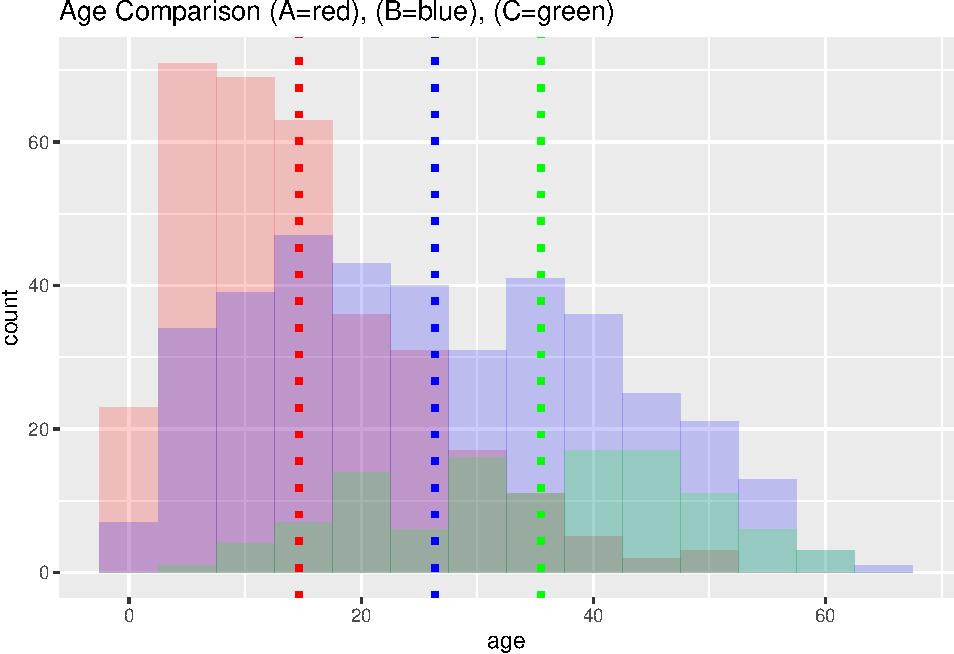
\includegraphics{final_files/figure-latex/unnamed-chunk-22-1.pdf}

The mean time since PhD completion of signers of Letter A is 14.6435
years and the median time is 13 years. The mean time since PhD
completion of signers of Letter B is 26.35433 years and the median time
is 24 years. The mean time since PhD completion of signers of Letter C
is 35.48 years and the median time is 37 years.

So signers of Letter C seem to be older than signers of Letter B, who in
turn seem older than signers of letter A. Let's validate this using a
permutation test.

\begin{Shaded}
\begin{Highlighting}[]
\NormalTok{muA <-}\StringTok{ }\KeywordTok{mean}\NormalTok{(}\KeywordTok{filter}\NormalTok{(df, (lettergroup }\OperatorTok{==}\StringTok{ "A Only"}\OperatorTok{|}\NormalTok{lettergroup }\OperatorTok{==}\StringTok{ "A and B"}\NormalTok{))}\OperatorTok{$}\NormalTok{age, }\DataTypeTok{na.rm =} \OtherTok{TRUE}\NormalTok{)}
\NormalTok{muB <-}\StringTok{ }\KeywordTok{mean}\NormalTok{(}\KeywordTok{filter}\NormalTok{(df, (lettergroup }\OperatorTok{==}\StringTok{ "B Only"}\OperatorTok{|}\NormalTok{lettergroup }\OperatorTok{==}\StringTok{ "A and B"}\NormalTok{))}\OperatorTok{$}\NormalTok{age, }\DataTypeTok{na.rm =} \OtherTok{TRUE}\NormalTok{)}
\NormalTok{muC <-}\StringTok{ }\KeywordTok{mean}\NormalTok{(}\KeywordTok{filter}\NormalTok{(df, (lettergroup }\OperatorTok{==}\StringTok{ "C Only"}\OperatorTok{|}\NormalTok{lettergroup }\OperatorTok{==}\StringTok{ "B and C"}\NormalTok{))}\OperatorTok{$}\NormalTok{age, }\DataTypeTok{na.rm =} \OtherTok{TRUE}\NormalTok{)}

\NormalTok{val1 <-}\StringTok{ }\NormalTok{muA }\OperatorTok{-}\StringTok{ }\NormalTok{muB}
\NormalTok{val2 <-}\StringTok{ }\NormalTok{muB }\OperatorTok{-}\StringTok{ }\NormalTok{muC}
\NormalTok{val3 <-}\StringTok{ }\NormalTok{muA }\OperatorTok{-}\StringTok{ }\NormalTok{muC}
\KeywordTok{set.seed}\NormalTok{(}\DecValTok{0}\NormalTok{)}
\NormalTok{dist <-}\StringTok{ }\KeywordTok{meanPermutation}\NormalTok{(}\KeywordTok{na.omit}\NormalTok{(df}\OperatorTok{$}\NormalTok{age,}\DataTypeTok{cols=}\StringTok{"age"}\NormalTok{),}\DecValTok{10000}\NormalTok{)}

\KeywordTok{hist}\NormalTok{(dist,}
     \DataTypeTok{main =} \StringTok{"Age"}\NormalTok{,}
     \DataTypeTok{xlab =} \StringTok{"Differences in Mean"}\NormalTok{)}
\KeywordTok{abline}\NormalTok{(}\DataTypeTok{v=}\NormalTok{val1, }\DataTypeTok{col =} \StringTok{"red"}\NormalTok{)}
\KeywordTok{abline}\NormalTok{(}\DataTypeTok{v=}\NormalTok{val2, }\DataTypeTok{col =} \StringTok{"blue"}\NormalTok{)}
\KeywordTok{abline}\NormalTok{(}\DataTypeTok{v=}\NormalTok{val3, }\DataTypeTok{col =} \StringTok{"green"}\NormalTok{)}
\end{Highlighting}
\end{Shaded}

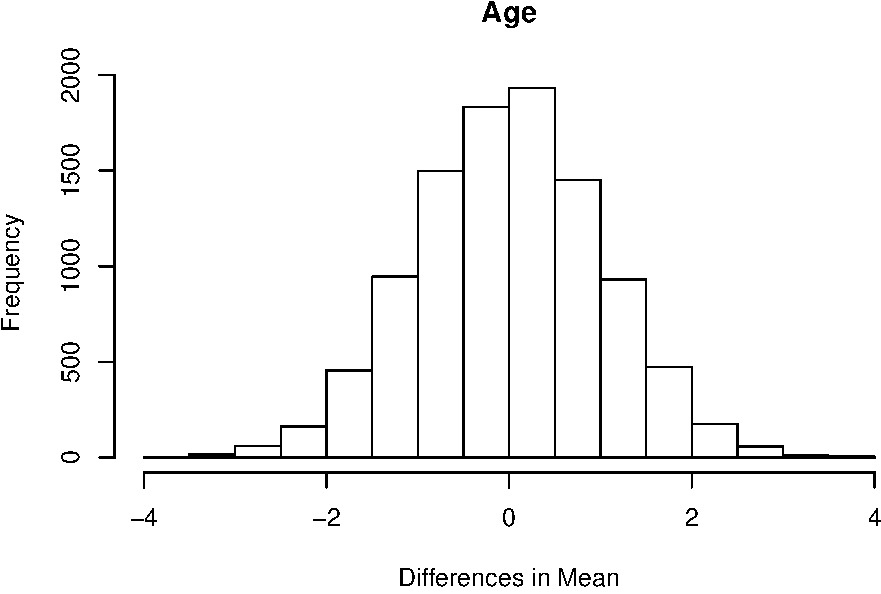
\includegraphics{final_files/figure-latex/unnamed-chunk-24-1.pdf}

All three differences in mean age lie outside of the induced
distribution, so it is unlikely that the observed differences were due
to chance, and we can reject all three null hypotheses.

\hypertarget{citations}{%
\subsection{Citations}\label{citations}}

How do the number of citations compare amongst signers of letter A, B,
and C? This is a trickier question, because many things influence how
many citations a researcher has - age and field for instance - and the
number of citations differ between Google Scholar, which includes
preprints, and MathSciNet, which only includes published papers. We will
subset accordingly, and run permutation tests on each to validate.

\hypertarget{math-sci-net-citations}{%
\subsubsection{Math Sci Net citations}\label{math-sci-net-citations}}

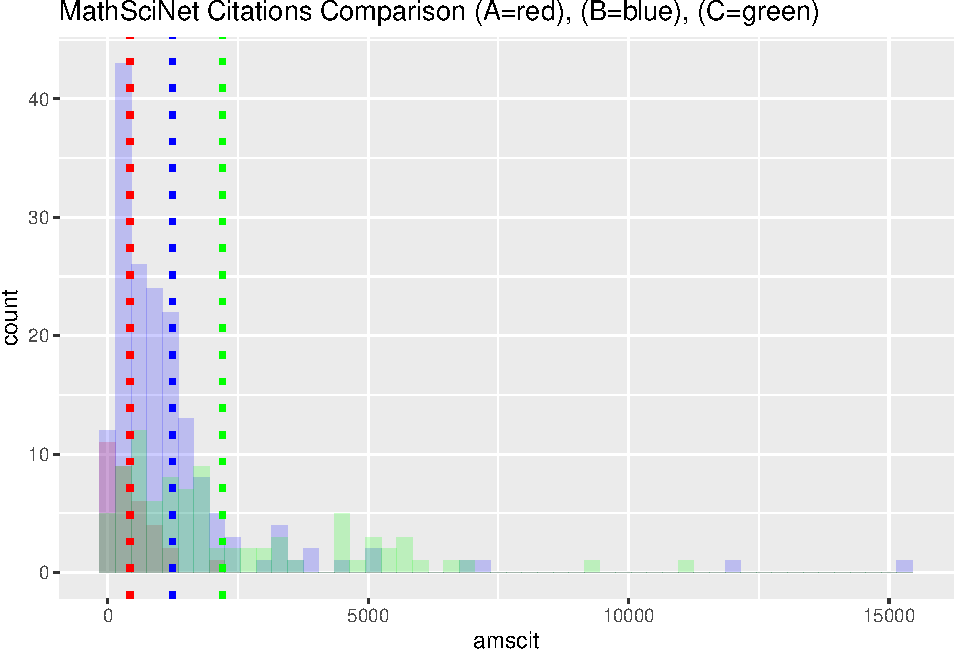
\includegraphics{final_files/figure-latex/unnamed-chunk-25-1.pdf}

Using Math Sci Net, the mean number of citations for signers of Letter A
is 424.64, and the median is 299. The mean number of citations for
signers of Letter B is 1312.50, and the median is 866. The mean number
of citations for signers of Letter C is 2204.74, and the median is
1392.5. So it seems by directly comparing populations, signers of Letter
A had less citations than their counterparts on B and C. Let's validate
this using a permutation test.

\begin{Shaded}
\begin{Highlighting}[]
\NormalTok{muA <-}\StringTok{ }\KeywordTok{mean}\NormalTok{(}\KeywordTok{filter}\NormalTok{(df, (lettergroup }\OperatorTok{==}\StringTok{ "A Only"}\OperatorTok{|}\NormalTok{lettergroup }\OperatorTok{==}\StringTok{ "A and B"}\NormalTok{))}\OperatorTok{$}\NormalTok{amscit, }\DataTypeTok{na.rm =} \OtherTok{TRUE}\NormalTok{)}
\NormalTok{muB <-}\StringTok{ }\KeywordTok{mean}\NormalTok{(}\KeywordTok{filter}\NormalTok{(df, (lettergroup }\OperatorTok{==}\StringTok{ "B Only"}\OperatorTok{|}\NormalTok{lettergroup }\OperatorTok{==}\StringTok{ "A and B"}\NormalTok{))}\OperatorTok{$}\NormalTok{amscit, }\DataTypeTok{na.rm =} \OtherTok{TRUE}\NormalTok{)}
\NormalTok{muC <-}\StringTok{ }\KeywordTok{mean}\NormalTok{(}\KeywordTok{filter}\NormalTok{(df, (lettergroup }\OperatorTok{==}\StringTok{ "C Only"}\OperatorTok{|}\NormalTok{lettergroup }\OperatorTok{==}\StringTok{ "B and C"}\NormalTok{))}\OperatorTok{$}\NormalTok{amscit, }\DataTypeTok{na.rm =} \OtherTok{TRUE}\NormalTok{)}

\NormalTok{val1 <-}\StringTok{ }\NormalTok{muA }\OperatorTok{-}\StringTok{ }\NormalTok{muB}
\NormalTok{val2 <-}\StringTok{ }\NormalTok{muB }\OperatorTok{-}\StringTok{ }\NormalTok{muC}
\NormalTok{val3 <-}\StringTok{ }\NormalTok{muA }\OperatorTok{-}\StringTok{ }\NormalTok{muC}

\NormalTok{dist <-}\StringTok{ }\KeywordTok{meanPermutation}\NormalTok{(}\KeywordTok{na.omit}\NormalTok{(df}\OperatorTok{$}\NormalTok{amscit),}\DecValTok{10000}\NormalTok{)}
\KeywordTok{set.seed}\NormalTok{(}\DecValTok{0}\NormalTok{)}

\KeywordTok{hist}\NormalTok{(dist,}
     \DataTypeTok{main =} \StringTok{"Permutation Test on MathSciNet citations"}\NormalTok{,}
     \DataTypeTok{xlab =} \StringTok{"Differences in Mean"}\NormalTok{)}
\KeywordTok{abline}\NormalTok{(}\DataTypeTok{v=}\NormalTok{val1, }\DataTypeTok{col =} \StringTok{"red"}\NormalTok{)}
\KeywordTok{abline}\NormalTok{(}\DataTypeTok{v=}\NormalTok{val2, }\DataTypeTok{col =} \StringTok{"blue"}\NormalTok{)}
\KeywordTok{abline}\NormalTok{(}\DataTypeTok{v=}\NormalTok{val3, }\DataTypeTok{col =} \StringTok{"green"}\NormalTok{)}
\end{Highlighting}
\end{Shaded}

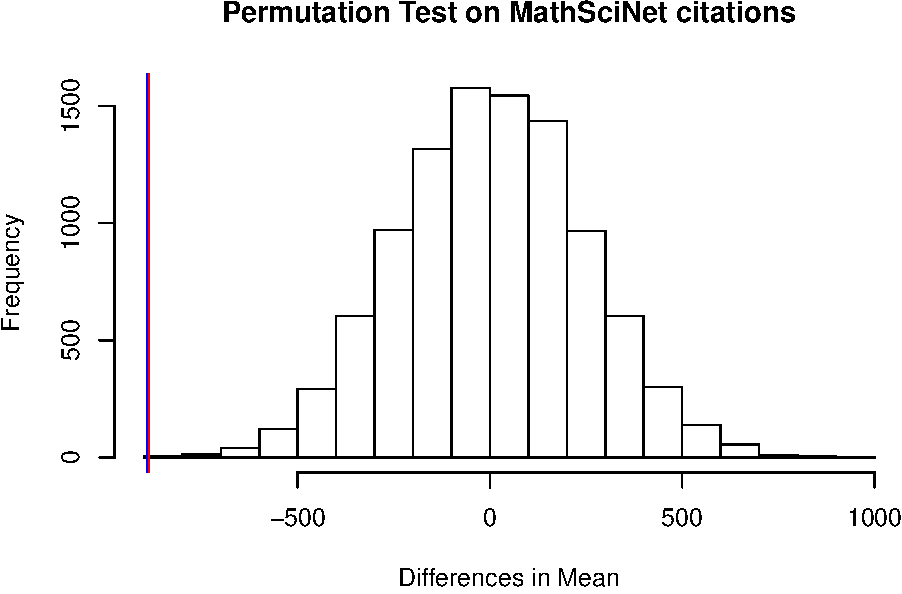
\includegraphics{final_files/figure-latex/unnamed-chunk-27-1.pdf}

The probability that the difference in mean number of citations between
signers of A and B is 0.01\%. The difference between B and C and A and C
are both outside the induced distribution. So it is unlikely that the
observed difference in the number of MathSciNet citations was due to
chance, and we may reject all three null hypotheses.

\hypertarget{mathscinet-citations-only-professors}{%
\subsubsection{MathSciNet Citations Only
Professors}\label{mathscinet-citations-only-professors}}

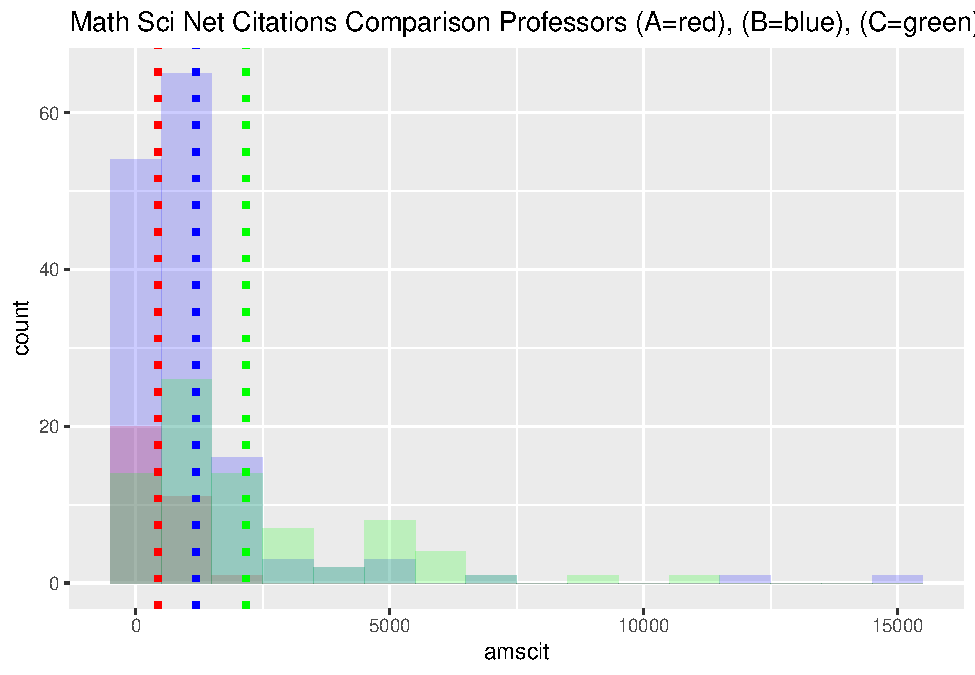
\includegraphics{final_files/figure-latex/unnamed-chunk-29-1.pdf}

The mean number of citations on Mathscinet for professors who were
signers of Letter A is 437.91, and the median is 300. The mean number of
citations for professors who were signers of Letter B is 1182.27, and
the median is 728.5. The mean number of citations for professors who
were signers of Letter C is 2176.64, and the median is 1353.

So it seems by directly comparing populations, signers of Letter A had
less citations than their counterparts on B and C. Let's validate this
using a permutation test.

\begin{Shaded}
\begin{Highlighting}[]
\NormalTok{muA <-}\StringTok{ }\KeywordTok{mean}\NormalTok{(}\KeywordTok{filter}\NormalTok{(df, ((lettergroup }\OperatorTok{==}\StringTok{ "A Only"}\OperatorTok{|}\NormalTok{lettergroup }\OperatorTok{==}\StringTok{ "A and B"}\NormalTok{)}\OperatorTok{&}\NormalTok{(role}\OperatorTok{==}\StringTok{"professor"}\NormalTok{)))}\OperatorTok{$}\NormalTok{amscit, }\DataTypeTok{na.rm =} \OtherTok{TRUE}\NormalTok{)}
\NormalTok{muB <-}\StringTok{ }\KeywordTok{mean}\NormalTok{(}\KeywordTok{filter}\NormalTok{(df, ((lettergroup }\OperatorTok{==}\StringTok{ "B Only"}\OperatorTok{|}\NormalTok{lettergroup }\OperatorTok{==}\StringTok{ "A and B"}\NormalTok{)}\OperatorTok{&}\NormalTok{(role}\OperatorTok{==}\StringTok{"professor"}\NormalTok{)))}\OperatorTok{$}\NormalTok{amscit, }\DataTypeTok{na.rm =} \OtherTok{TRUE}\NormalTok{)}
\NormalTok{muC <-}\StringTok{ }\KeywordTok{mean}\NormalTok{(}\KeywordTok{filter}\NormalTok{(df, ((lettergroup }\OperatorTok{==}\StringTok{ "C Only"}\OperatorTok{|}\NormalTok{lettergroup }\OperatorTok{==}\StringTok{ "B and C"}\NormalTok{)}\OperatorTok{&}\NormalTok{(role}\OperatorTok{==}\StringTok{"professor"}\NormalTok{)))}\OperatorTok{$}\NormalTok{amscit, }\DataTypeTok{na.rm =} \OtherTok{TRUE}\NormalTok{)}

\NormalTok{val1 <-}\StringTok{ }\NormalTok{muA }\OperatorTok{-}\StringTok{ }\NormalTok{muB}
\NormalTok{val2 <-}\StringTok{ }\NormalTok{muB }\OperatorTok{-}\StringTok{ }\NormalTok{muC}
\NormalTok{val3 <-}\StringTok{ }\NormalTok{muA }\OperatorTok{-}\StringTok{ }\NormalTok{muC}

\KeywordTok{set.seed}\NormalTok{(}\DecValTok{0}\NormalTok{)}
\NormalTok{dist <-}\StringTok{ }\KeywordTok{meanPermutation}\NormalTok{(}\KeywordTok{na.omit}\NormalTok{(df}\OperatorTok{$}\NormalTok{amscit),}\DecValTok{10000}\NormalTok{)}

\KeywordTok{hist}\NormalTok{(dist,}
     \DataTypeTok{main =} \StringTok{"Permutation Test on MathSciNet citations only professors"}\NormalTok{,}
     \DataTypeTok{xlab =} \StringTok{"Differences in Mean"}\NormalTok{)}
\KeywordTok{abline}\NormalTok{(}\DataTypeTok{v=}\NormalTok{val1, }\DataTypeTok{col =} \StringTok{"red"}\NormalTok{)}
\KeywordTok{abline}\NormalTok{(}\DataTypeTok{v=}\NormalTok{val2, }\DataTypeTok{col =} \StringTok{"blue"}\NormalTok{)}
\KeywordTok{abline}\NormalTok{(}\DataTypeTok{v=}\NormalTok{val3, }\DataTypeTok{col =} \StringTok{"green"}\NormalTok{)}
\end{Highlighting}
\end{Shaded}

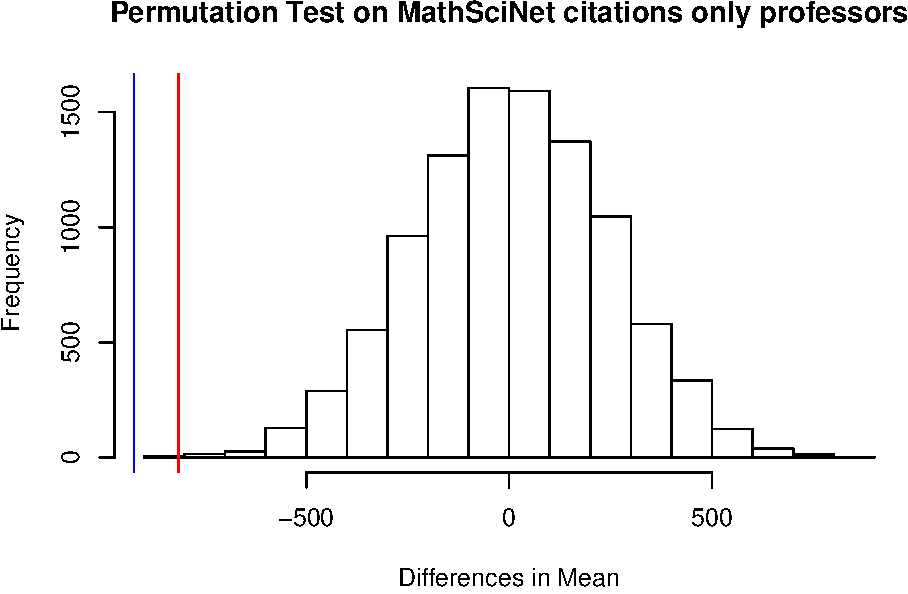
\includegraphics{final_files/figure-latex/unnamed-chunk-31-1.pdf}

All observed differences lie outside the induced distribution, so it is
unlikely the observed differences were due to chance. Accordingly, we
may reject all three null hypotheses.

\hypertarget{mathscinet-citations-per-year}{%
\subsubsection{MathSciNet Citations per
Year}\label{mathscinet-citations-per-year}}

Older researchers have had a longer time to rack up citations, so it is
important to normalize for this and divide by the length of time
professionals have had their PhDs.

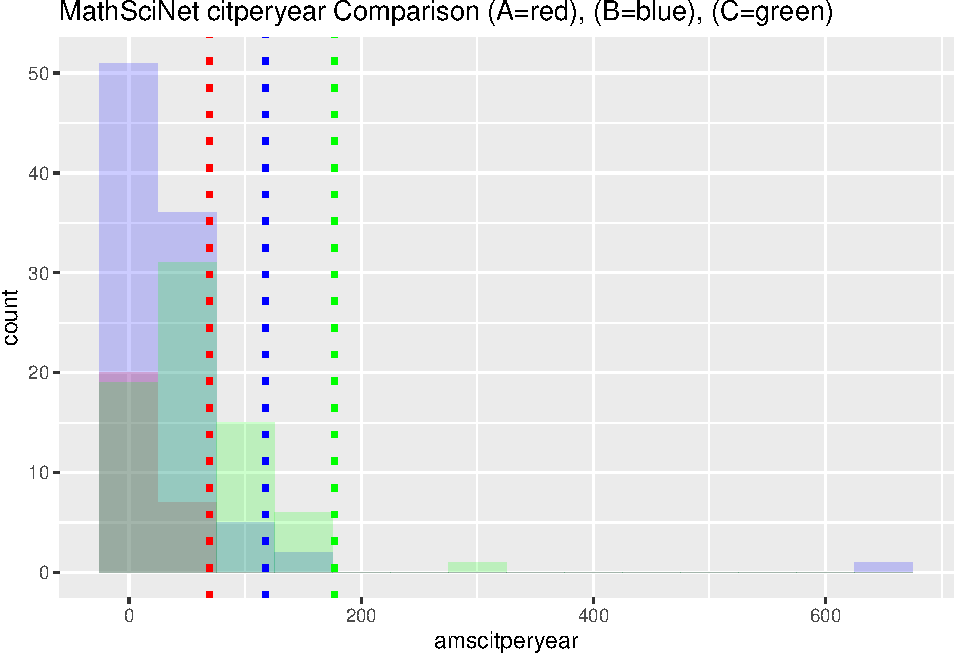
\includegraphics{final_files/figure-latex/unnamed-chunk-33-1.pdf}

The mean number of citations per year for signers of Letter A is 16.88,
and the median is 13.08. The mean number of citations per year for
signers of Letter B is 37.22, and the median is 24.15. The mean number
of citations per year for signers of Letter C is 55.55, and the median
is 42.42.

So it seems by directly comparing populations, professors on Letter A
had less citations per year than their counterparts on B and C. Let's
validate this using a permutation test.

\begin{Shaded}
\begin{Highlighting}[]
\NormalTok{muA <-}\StringTok{ }\KeywordTok{mean}\NormalTok{(}\KeywordTok{filter}\NormalTok{(df, (lettergroup }\OperatorTok{==}\StringTok{ "A Only"}\OperatorTok{|}\NormalTok{lettergroup }\OperatorTok{==}\StringTok{ "A and B"}\NormalTok{))}\OperatorTok{$}\NormalTok{amscitperyear, }\DataTypeTok{na.rm =} \OtherTok{TRUE}\NormalTok{)}
\NormalTok{muB <-}\StringTok{ }\KeywordTok{mean}\NormalTok{(}\KeywordTok{filter}\NormalTok{(df, (lettergroup }\OperatorTok{==}\StringTok{ "B Only"}\OperatorTok{|}\NormalTok{lettergroup }\OperatorTok{==}\StringTok{ "A and B"}\NormalTok{))}\OperatorTok{$}\NormalTok{amscitperyear, }\DataTypeTok{na.rm =} \OtherTok{TRUE}\NormalTok{)}
\NormalTok{muC <-}\StringTok{ }\KeywordTok{mean}\NormalTok{(}\KeywordTok{filter}\NormalTok{(df, (lettergroup }\OperatorTok{==}\StringTok{ "C Only"}\OperatorTok{|}\NormalTok{lettergroup }\OperatorTok{==}\StringTok{ "B and C"}\NormalTok{))}\OperatorTok{$}\NormalTok{amscitperyear, }\DataTypeTok{na.rm =} \OtherTok{TRUE}\NormalTok{)}

\NormalTok{val1 <-}\StringTok{ }\NormalTok{muA }\OperatorTok{-}\StringTok{ }\NormalTok{muB}
\NormalTok{val2 <-}\StringTok{ }\NormalTok{muB }\OperatorTok{-}\StringTok{ }\NormalTok{muC}
\NormalTok{val3 <-}\StringTok{ }\NormalTok{muA }\OperatorTok{-}\StringTok{ }\NormalTok{muC}

\KeywordTok{set.seed}\NormalTok{(}\DecValTok{0}\NormalTok{)}
\NormalTok{dist <-}\StringTok{ }\KeywordTok{meanPermutation}\NormalTok{(}\KeywordTok{na.omit}\NormalTok{(df}\OperatorTok{$}\NormalTok{amscitperyear),}\DecValTok{10000}\NormalTok{)}

\KeywordTok{hist}\NormalTok{(dist,}
     \DataTypeTok{main =} \StringTok{"Citations per Year Math Sci Net"}\NormalTok{,}
     \DataTypeTok{xlab =} \StringTok{"Differences in Mean"}\NormalTok{)}
\KeywordTok{abline}\NormalTok{(}\DataTypeTok{v=}\NormalTok{val1, }\DataTypeTok{col =} \StringTok{"red"}\NormalTok{)}
\KeywordTok{abline}\NormalTok{(}\DataTypeTok{v=}\NormalTok{val2, }\DataTypeTok{col =} \StringTok{"blue"}\NormalTok{)}
\KeywordTok{abline}\NormalTok{(}\DataTypeTok{v=}\NormalTok{val3, }\DataTypeTok{col =} \StringTok{"green"}\NormalTok{)}
\end{Highlighting}
\end{Shaded}

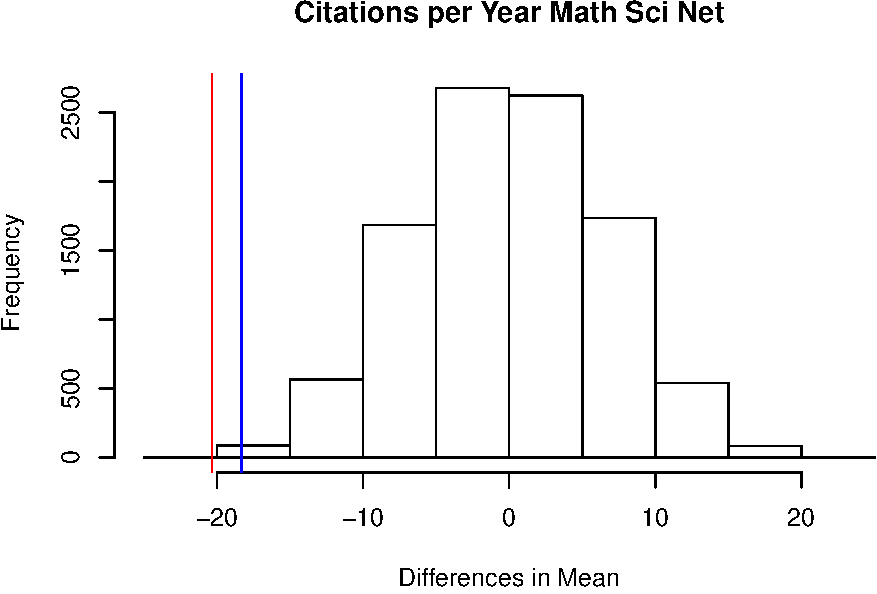
\includegraphics{final_files/figure-latex/unnamed-chunk-35-1.pdf}

\begin{verbatim}
## [1] 4e-04
\end{verbatim}

\begin{verbatim}
## [1] 0.0084
\end{verbatim}

\begin{verbatim}
## [1] 0
\end{verbatim}

The percentage of the induced distribution that is more extreme than the
observed difference in mean number of citations per year between A and B
is .03\%. The percentage of the induced distribution that is more
extreme than the observed difference in mean number of citations per
year between B and C is .18\%.The observed difference in mean between A
and C is outside the induced distribution. So it is unlikely that the
observed difference in the number of Google Scholar citations was due to
chance, and we may reject all three null hypotheses.

\hypertarget{mathscinet-citations-per-year-only-professors}{%
\subsubsection{MathSciNet Citations per Year only
professors}\label{mathscinet-citations-per-year-only-professors}}

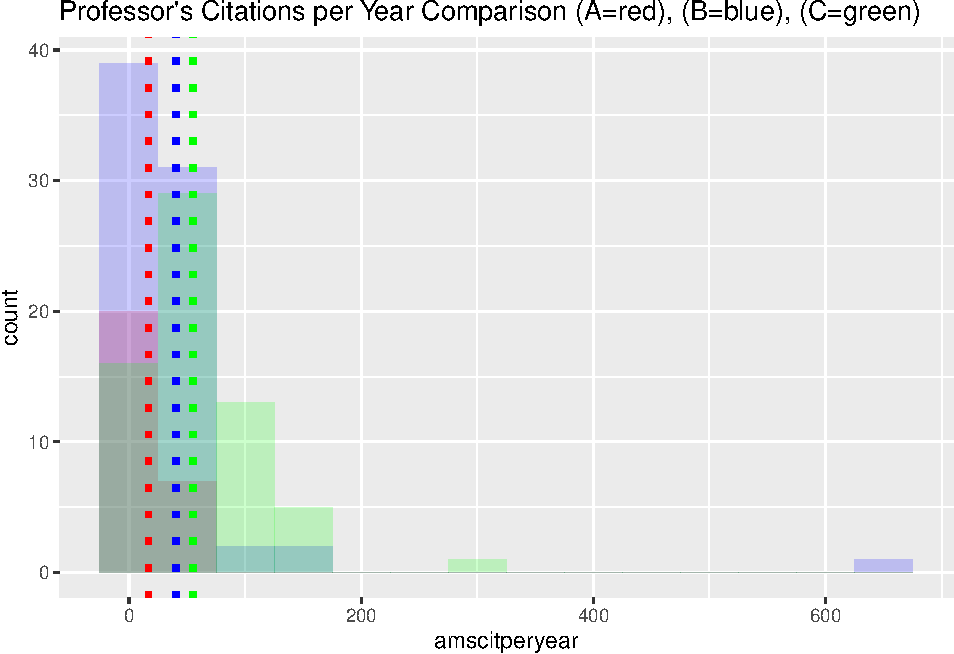
\includegraphics{final_files/figure-latex/unnamed-chunk-37-1.pdf}

The mean number of citations per year for professors who were signers of
Letter A is 16.88, and the median is 13.08. The mean number of citations
per year for professors who were signers of Letter B is 38.05, and the
median is 24.15. The mean number of citations per year for professors
who were signers of Letter C is 55.36, and the median is 41.74.

So it seems when comparing only professors, signers of Letter A had less
citations than their counterparts on B and C. Let's validate this using
a permutation test.

\begin{Shaded}
\begin{Highlighting}[]
\NormalTok{muA <-}\StringTok{ }\KeywordTok{mean}\NormalTok{(}\KeywordTok{filter}\NormalTok{(df, ((lettergroup }\OperatorTok{==}\StringTok{ "A Only"}\OperatorTok{|}\NormalTok{lettergroup }\OperatorTok{==}\StringTok{ "A and B"}\NormalTok{)}\OperatorTok{&}\NormalTok{(role}\OperatorTok{==}\StringTok{"professor"}\NormalTok{)))}\OperatorTok{$}\NormalTok{amscitperyear, }\DataTypeTok{na.rm =} \OtherTok{TRUE}\NormalTok{)}
\NormalTok{muB <-}\StringTok{ }\KeywordTok{mean}\NormalTok{(}\KeywordTok{filter}\NormalTok{(df, ((lettergroup }\OperatorTok{==}\StringTok{ "B Only"}\OperatorTok{|}\NormalTok{lettergroup }\OperatorTok{==}\StringTok{ "A and B"}\NormalTok{)}\OperatorTok{&}\NormalTok{(role}\OperatorTok{==}\StringTok{"professor"}\NormalTok{)))}\OperatorTok{$}\NormalTok{amscitperyear, }\DataTypeTok{na.rm =} \OtherTok{TRUE}\NormalTok{)}
\NormalTok{muC <-}\StringTok{ }\KeywordTok{mean}\NormalTok{(}\KeywordTok{filter}\NormalTok{(df, ((lettergroup }\OperatorTok{==}\StringTok{ "C Only"}\OperatorTok{|}\NormalTok{lettergroup }\OperatorTok{==}\StringTok{ "B and C"}\NormalTok{)}\OperatorTok{&}\NormalTok{(role}\OperatorTok{==}\StringTok{"professor"}\NormalTok{)))}\OperatorTok{$}\NormalTok{amscitperyear, }\DataTypeTok{na.rm =} \OtherTok{TRUE}\NormalTok{)}

\NormalTok{val1 <-}\StringTok{ }\NormalTok{muA}\OperatorTok{-}\NormalTok{muB}
\NormalTok{val2 <-}\StringTok{ }\NormalTok{muB }\OperatorTok{-}\StringTok{ }\NormalTok{muC}
\NormalTok{val3 <-}\StringTok{ }\NormalTok{muA }\OperatorTok{-}\StringTok{ }\NormalTok{muC}

\KeywordTok{set.seed}\NormalTok{(}\DecValTok{0}\NormalTok{)}
\NormalTok{dist <-}\StringTok{ }\KeywordTok{meanPermutation}\NormalTok{(}\KeywordTok{na.omit}\NormalTok{(df}\OperatorTok{$}\NormalTok{amscitperyear),}\DecValTok{10000}\NormalTok{)}

\KeywordTok{hist}\NormalTok{(dist,}
     \DataTypeTok{main =} \StringTok{"AMS citations per year permutation test"}\NormalTok{,}
     \DataTypeTok{xlab =} \StringTok{"Differences in Mean"}\NormalTok{)}
\KeywordTok{abline}\NormalTok{(}\DataTypeTok{v=}\NormalTok{val1, }\DataTypeTok{col =} \StringTok{"red"}\NormalTok{)}
\KeywordTok{abline}\NormalTok{(}\DataTypeTok{v=}\NormalTok{val2, }\DataTypeTok{col =} \StringTok{"blue"}\NormalTok{)}
\KeywordTok{abline}\NormalTok{(}\DataTypeTok{v=}\NormalTok{val3, }\DataTypeTok{col =} \StringTok{"green"}\NormalTok{)}
\end{Highlighting}
\end{Shaded}

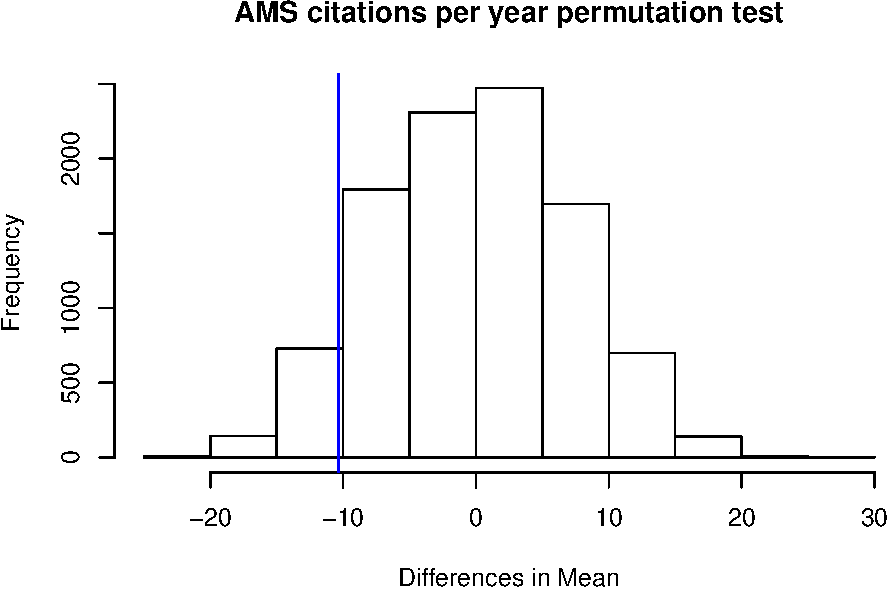
\includegraphics{final_files/figure-latex/unnamed-chunk-39-1.pdf}

About 0.02\% of the induced distribution is more extreme than the
observed difference between A and B, so it is highly unlikely the
observed difference was due to chance. Only 0.34\% of the induced
distribution was more extreme than the difference between B and C, and
0\% between A and C, so it is unlikely those were due to chance. We may
reject all three null hypotheses.

\hypertarget{ams-citations-per-year---female-professors-only}{%
\subsubsection{AMS Citations Per Year - Female Professors
Only}\label{ams-citations-per-year---female-professors-only}}

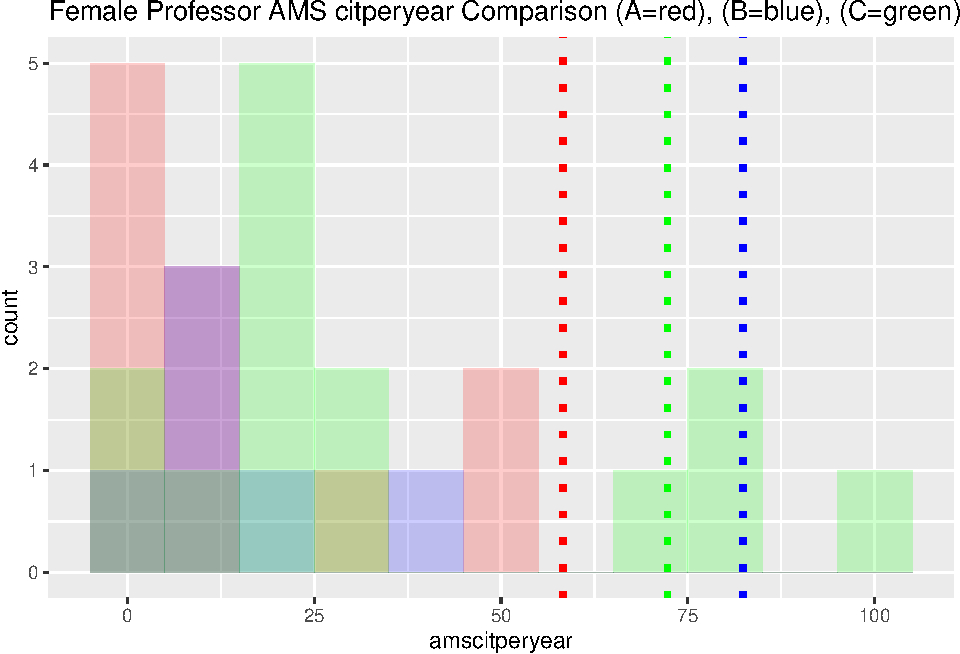
\includegraphics{final_files/figure-latex/unnamed-chunk-41-1.pdf}

Using the data from mathscinet, the mean number of citations per year
for female professors who were signers of Letter A is 15.30, and the
median is 5.55. The mean number of citations per year for female
professors who were signers of Letter B is 22.54, and the median is
14.80. The mean number of citations per year for female professors who
were signers of Letter C is 35.04, and the median is 22.70.

So it seems when comparing only female professors, signers of Letter A
had less citations than their counterparts on B and C.

Let's validate this using a permutation test.

\begin{Shaded}
\begin{Highlighting}[]
\NormalTok{muA <-}\StringTok{ }\KeywordTok{mean}\NormalTok{(}\KeywordTok{filter}\NormalTok{(df, ((lettergroup }\OperatorTok{==}\StringTok{ "A Only"}\OperatorTok{|}\NormalTok{lettergroup }\OperatorTok{==}\StringTok{ "A and B"}\NormalTok{)}\OperatorTok{&}\NormalTok{(role}\OperatorTok{==}\StringTok{"professor"}\NormalTok{)}\OperatorTok{&}\NormalTok{(gender}\OperatorTok{==}\StringTok{"woman"}\NormalTok{)))}\OperatorTok{$}\NormalTok{amscitperyear, }\DataTypeTok{na.rm =} \OtherTok{TRUE}\NormalTok{)}
\NormalTok{muB <-}\StringTok{ }\KeywordTok{mean}\NormalTok{(}\KeywordTok{filter}\NormalTok{(df, ((lettergroup }\OperatorTok{==}\StringTok{ "B Only"}\OperatorTok{|}\NormalTok{lettergroup }\OperatorTok{==}\StringTok{ "A and B"}\NormalTok{)}\OperatorTok{&}\NormalTok{(role}\OperatorTok{==}\StringTok{"professor"}\NormalTok{)}\OperatorTok{&}\NormalTok{(gender}\OperatorTok{==}\StringTok{"woman"}\NormalTok{)))}\OperatorTok{$}\NormalTok{amscitperyear, }\DataTypeTok{na.rm =} \OtherTok{TRUE}\NormalTok{)}
\NormalTok{muC <-}\StringTok{ }\KeywordTok{mean}\NormalTok{(}\KeywordTok{filter}\NormalTok{(df, ((lettergroup }\OperatorTok{==}\StringTok{ "C Only"}\OperatorTok{|}\NormalTok{lettergroup }\OperatorTok{==}\StringTok{ "B and C"}\NormalTok{)}\OperatorTok{&}\NormalTok{(role}\OperatorTok{==}\StringTok{"professor"}\NormalTok{)}\OperatorTok{&}\NormalTok{(gender}\OperatorTok{==}\StringTok{"woman"}\NormalTok{)))}\OperatorTok{$}\NormalTok{amscitperyear, }\DataTypeTok{na.rm =} \OtherTok{TRUE}\NormalTok{)}

\NormalTok{val1 <-}\StringTok{ }\NormalTok{muA }\OperatorTok{-}\StringTok{ }\NormalTok{muB}
\NormalTok{val2 <-}\StringTok{ }\NormalTok{muB }\OperatorTok{-}\StringTok{ }\NormalTok{muC}
\NormalTok{val3 <-}\StringTok{ }\NormalTok{muA }\OperatorTok{-}\StringTok{ }\NormalTok{muC}

\KeywordTok{set.seed}\NormalTok{(}\DecValTok{0}\NormalTok{)}


\NormalTok{dist <-}\StringTok{ }\KeywordTok{meanPermutation}\NormalTok{(}\KeywordTok{na.omit}\NormalTok{(}\KeywordTok{filter}\NormalTok{(df, ((gender}\OperatorTok{==}\StringTok{"woman"}\NormalTok{)}\OperatorTok{&}\NormalTok{(role}\OperatorTok{==}\StringTok{"professor"}\NormalTok{)))}\OperatorTok{$}\NormalTok{amscitperyear),}\DecValTok{10000}\NormalTok{)}

\KeywordTok{hist}\NormalTok{(dist,}
     \DataTypeTok{main =} \StringTok{"MathSciNet citperyear Female Professors"}\NormalTok{,}
     \DataTypeTok{xlab =} \StringTok{"Differences in Mean"}\NormalTok{)}
\KeywordTok{abline}\NormalTok{(}\DataTypeTok{v=}\NormalTok{val1, }\DataTypeTok{col =} \StringTok{"red"}\NormalTok{)}
\KeywordTok{abline}\NormalTok{(}\DataTypeTok{v=}\NormalTok{val2, }\DataTypeTok{col =} \StringTok{"blue"}\NormalTok{)}
\KeywordTok{abline}\NormalTok{(}\DataTypeTok{v=}\NormalTok{val3, }\DataTypeTok{col =} \StringTok{"green"}\NormalTok{)}
\end{Highlighting}
\end{Shaded}

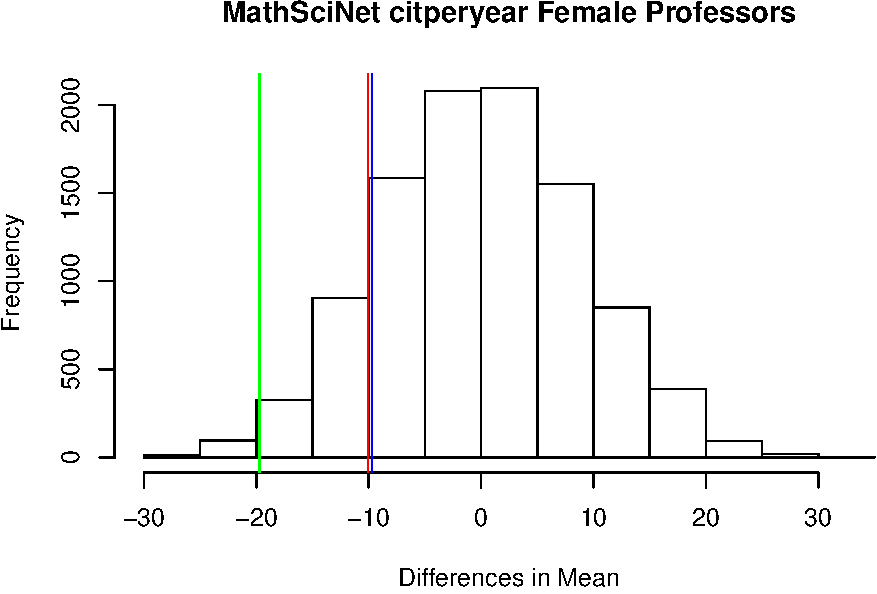
\includegraphics{final_files/figure-latex/unnamed-chunk-43-1.pdf}

20.37\% of the induced distribution was more extreme than the observed
difference in mean between A and B. 7.38\% of the induced distribution
was more extreme than the observed difference in mean between B and C.
0.88\% of the induced distribution was more extreme than the observed
difference in ean between A and C. We fail to reject the difference in
mean between female professors of Letter A and B, but we may reject the
null hypothesis for the difference in citations per year for female
signers of B and C, and C and A.

\hypertarget{hindex}{%
\subsection{hindex}\label{hindex}}

An h-index is an alternative metric to citations to assess author
impact. It attempts to balance the number of published papers and the
number of citations.

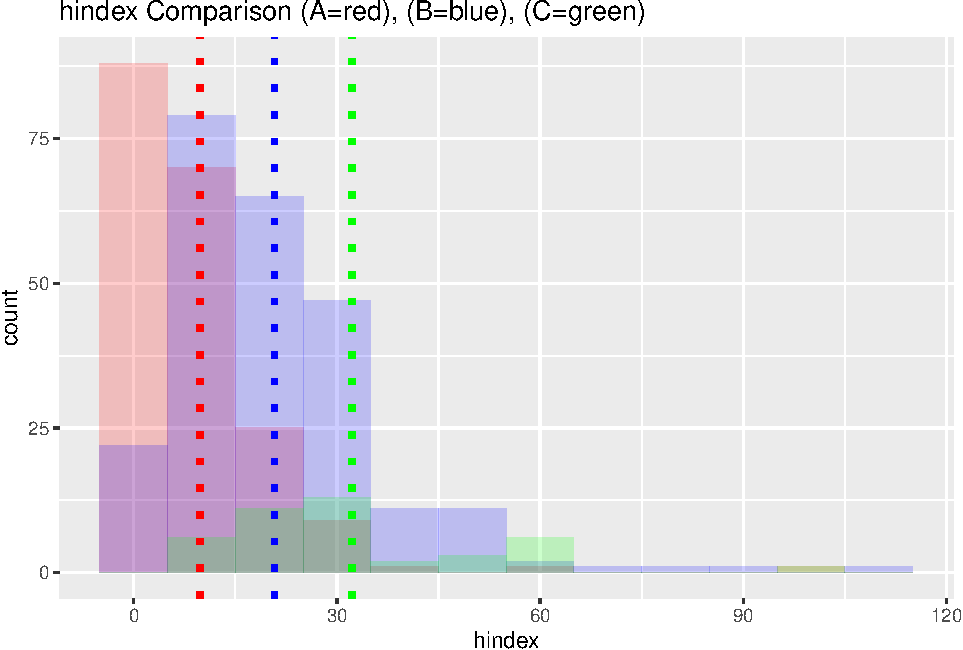
\includegraphics{final_files/figure-latex/unnamed-chunk-45-1.pdf}

The mean number of h-index for signers of Letter A is 9.73, and the
median is 6. The mean number of h-index for signers of Letter B is
20.78, and the median is 17. The mean h-index for signers of Letter C is
32.24, and the median is 29.5.

It appears that the signers of letter A had a lower h-index than signers
of B and C. Let's assess this using a permutation test.

\begin{Shaded}
\begin{Highlighting}[]
\NormalTok{muA <-}\StringTok{ }\KeywordTok{mean}\NormalTok{(}\KeywordTok{filter}\NormalTok{(df, (lettergroup }\OperatorTok{==}\StringTok{ "A Only"}\OperatorTok{|}\NormalTok{lettergroup }\OperatorTok{==}\StringTok{ "A and B"}\NormalTok{))}\OperatorTok{$}\NormalTok{hindex, }\DataTypeTok{na.rm =} \OtherTok{TRUE}\NormalTok{)}
\NormalTok{muB <-}\StringTok{ }\KeywordTok{mean}\NormalTok{(}\KeywordTok{filter}\NormalTok{(df, (lettergroup }\OperatorTok{==}\StringTok{ "B Only"}\OperatorTok{|}\NormalTok{lettergroup }\OperatorTok{==}\StringTok{ "A and B"}\NormalTok{))}\OperatorTok{$}\NormalTok{hindex, }\DataTypeTok{na.rm =} \OtherTok{TRUE}\NormalTok{)}
\NormalTok{muC <-}\StringTok{ }\KeywordTok{mean}\NormalTok{(}\KeywordTok{filter}\NormalTok{(df, (lettergroup }\OperatorTok{==}\StringTok{ "C Only"}\OperatorTok{|}\NormalTok{lettergroup }\OperatorTok{==}\StringTok{ "B and C"}\NormalTok{))}\OperatorTok{$}\NormalTok{hindex, }\DataTypeTok{na.rm =} \OtherTok{TRUE}\NormalTok{)}

\NormalTok{val1 <-}\StringTok{ }\NormalTok{muA }\OperatorTok{-}\StringTok{ }\NormalTok{muB}
\NormalTok{val2 <-}\StringTok{ }\NormalTok{muB }\OperatorTok{-}\StringTok{ }\NormalTok{muC}
\NormalTok{val3 <-}\StringTok{ }\NormalTok{muA }\OperatorTok{-}\StringTok{ }\NormalTok{muC}

\NormalTok{dist <-}\StringTok{ }\KeywordTok{meanPermutation}\NormalTok{(}\KeywordTok{na.omit}\NormalTok{(df}\OperatorTok{$}\NormalTok{hindex,}\DataTypeTok{cols=}\StringTok{"hindex"}\NormalTok{),}\DecValTok{10000}\NormalTok{)}

\KeywordTok{hist}\NormalTok{(dist,}
     \DataTypeTok{main =} \StringTok{"hindex"}\NormalTok{,}
     \DataTypeTok{xlab =} \StringTok{"Differences in Mean"}\NormalTok{)}
\KeywordTok{abline}\NormalTok{(}\DataTypeTok{v=}\NormalTok{val1, }\DataTypeTok{col =} \StringTok{"red"}\NormalTok{)}
\KeywordTok{abline}\NormalTok{(}\DataTypeTok{v=}\NormalTok{val2, }\DataTypeTok{col =} \StringTok{"blue"}\NormalTok{)}
\KeywordTok{abline}\NormalTok{(}\DataTypeTok{v=}\NormalTok{val3, }\DataTypeTok{col =} \StringTok{"green"}\NormalTok{)}
\end{Highlighting}
\end{Shaded}

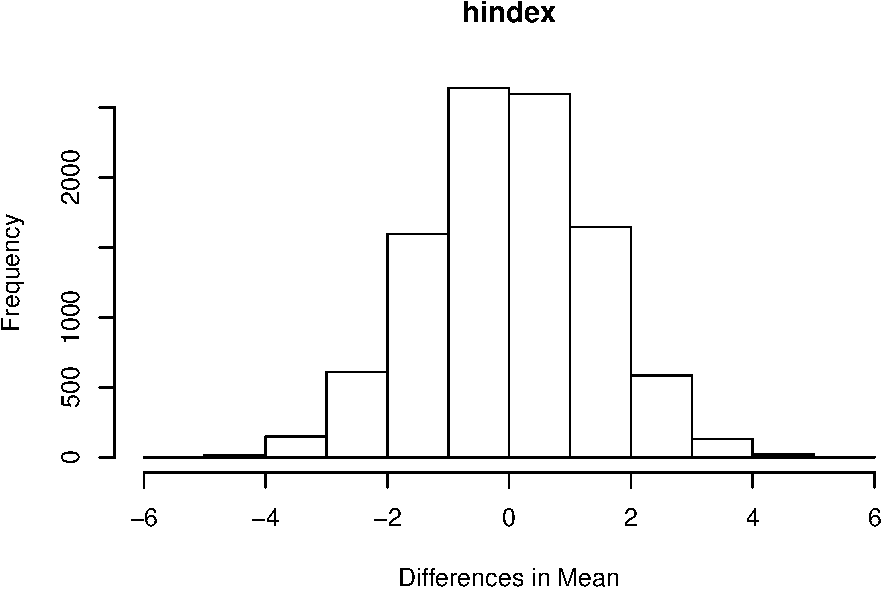
\includegraphics{final_files/figure-latex/unnamed-chunk-47-1.pdf}

All three differences in mean number of citations lie outside of the
induced distribution, so it is unlikely that the observed differences
were due to chance. We may hence reject the null hypothesis.

\hypertarget{control-rutgers-math-department}{%
\subsection{Control: Rutgers Math
Department}\label{control-rutgers-math-department}}

As a control, we look at the Google Scholar citations, the AMS
citations, respective citations per year, and h indices of the Rutger's
math department.

\begin{verbatim}
##      AMSCIT            phd       GoogleScholar      hindex    
##  Min.   : 120.0   Min.   :1955   Min.   : 367   Min.   :10.0  
##  1st Qu.: 566.5   1st Qu.:1976   1st Qu.:1150   1st Qu.:15.5  
##  Median : 846.0   Median :1985   Median :2630   Median :26.0  
##  Mean   :1297.2   Mean   :1984   Mean   :3393   Mean   :27.3  
##  3rd Qu.:1770.5   3rd Qu.:1992   3rd Qu.:4457   3rd Qu.:34.0  
##  Max.   :5219.0   Max.   :2005   Max.   :8452   Max.   :50.0  
##                                  NA's   :23     NA's   :23    
##       age          citperyear     amscitperyear    
##  Min.   :15.00   Min.   : 15.29   Min.   :  4.679  
##  1st Qu.:27.50   1st Qu.: 43.25   1st Qu.: 16.585  
##  Median :35.00   Median : 93.95   Median : 26.537  
##  Mean   :35.72   Mean   :101.75   Mean   : 35.007  
##  3rd Qu.:44.50   3rd Qu.:149.85   3rd Qu.: 48.162  
##  Max.   :65.00   Max.   :237.11   Max.   :136.286  
##                  NA's   :23
\end{verbatim}

The mean age for Rutger's faculty was 35.72 years. The mean h-index was
27.3. The mean Google Scholar citations was 3392.8. The mean AMS
citations is 1297.19. The mean Google Scholar citations per year is
101.75. The mean AMS citations is 35.01.

This is in line with signers of letter B, greater than signers of letter
A, and slightly less than that of signers of letter C.

\hypertarget{asian-and-eastern-european-born}{%
\subsection{Asian and Eastern European
Born}\label{asian-and-eastern-european-born}}

We are interested in the proportion of letter signers who are Math
Professors at R1 universities, who were born in Eastern European or
Asian Countries. We created this data by looking at Wikipedia's and
personal knowledge.

Summary Statistics.

\begin{verbatim}
##       China     Croatia       Czech      Greece     Hungary        Iran 
##          18           1           1           1           4           1 
##       Japan       Korea Netherlands      Poland     Romania      Russia 
##           1           1           1           3           7          67 
##      Serbia      Turkey        NA's 
##           2           2         246
\end{verbatim}

\begin{Shaded}
\begin{Highlighting}[]
\KeywordTok{table}\NormalTok{(}\KeywordTok{filter}\NormalTok{(df3, (Letter }\OperatorTok{==}\StringTok{ "A Only"}\OperatorTok{|}\NormalTok{Letter }\OperatorTok{==}\StringTok{ "A and B"}\NormalTok{))}\OperatorTok{$}\NormalTok{From)}
\end{Highlighting}
\end{Shaded}

\begin{verbatim}
## 
##       China     Croatia       Czech      Greece     Hungary        Iran 
##           0           0           0           0           0           0 
##       Japan       Korea Netherlands      Poland     Romania      Russia 
##           0           0           0           0           0           0 
##      Serbia      Turkey 
##           0           0
\end{verbatim}

No signers of Letter A who were Math Professors at R1 universities, were
from Eastern European or Asian Countries.

\begin{Shaded}
\begin{Highlighting}[]
\KeywordTok{table}\NormalTok{(}\KeywordTok{filter}\NormalTok{(df3, (Letter }\OperatorTok{==}\StringTok{ "B Only"}\OperatorTok{|}\NormalTok{Letter }\OperatorTok{==}\StringTok{ "A and B"}\NormalTok{))}\OperatorTok{$}\NormalTok{From)}
\end{Highlighting}
\end{Shaded}

\begin{verbatim}
## 
##       China     Croatia       Czech      Greece     Hungary        Iran 
##           6           1           0           0           0           1 
##       Japan       Korea Netherlands      Poland     Romania      Russia 
##           1           0           1           3           3          31 
##      Serbia      Turkey 
##           2           1
\end{verbatim}

Looking at signers of Letter B who were Math Professors at R1
universities, we find there were 6 native Chinese, 1 native Croatian, 1
native Iranian, 1 native Japanese, 1 native Dutch, 3 native Polacks, 3
native Romanians, 31 native Russians, 2 native Serbians, and 1 native
Turk.

\begin{Shaded}
\begin{Highlighting}[]
\KeywordTok{table}\NormalTok{(}\KeywordTok{filter}\NormalTok{(df3, (Letter }\OperatorTok{==}\StringTok{ "C Only"}\OperatorTok{|}\NormalTok{Letter }\OperatorTok{==}\StringTok{ "B and C"}\NormalTok{))}\OperatorTok{$}\NormalTok{From)}
\end{Highlighting}
\end{Shaded}

\begin{verbatim}
## 
##       China     Croatia       Czech      Greece     Hungary        Iran 
##          12           0           1           1           4           0 
##       Japan       Korea Netherlands      Poland     Romania      Russia 
##           0           1           0           0           4          36 
##      Serbia      Turkey 
##           0           1
\end{verbatim}

Looking at signers of Letter C who were Math Professors at R1
universities, we find there were 12 native Chinese, 1 native Czech, 1
native Greek, 4 native Hungarians, 1 native Korean, 4 native Romanians,
36 native Russians, and 1 native Turk.

\hypertarget{conclusion-and-discussion}{%
\section{Conclusion and Discussion}\label{conclusion-and-discussion}}

\hypertarget{bibliography}{%
\section{Bibliography}\label{bibliography}}

{[}1{]}
\url{https://www.ams.org/journals/notices/201911/rnoti-p1778.pdf}

{[}2{]} \url{https://www.ams.org/journals/notices/202001/rnoti-o1.pdf}

{[}3{]}
\url{https://qsideinstitute.org/2019/11/19/diversity-statements-in-hiring-the-american-mathematical-society-and-uc-davis/}

{[}4{]} \url{https://pypi.org/project/scholarly/}

{[}5{]} \url{https://scholar.google.com/}

{[}6{]} \url{https://genealogy.math.ndsu.nodak.edu/}

{[}7{]} \url{https://github.com/j2kun/math-genealogy-scraper}

{[}8{]} \url{https://qsideinstitute.org/download/ams-letters-study/}

{[}9{]}
\url{http://www.ams.org/profession/data/annual-survey/2016dp-tableDF1.pdf?fbclid=IwAR1mgI0qSEs5nCGquqye741_0lZU-ez7dlcJ3wZYhDtJUswhH1SX7yeiiak}

\hypertarget{appendix}{%
\section{Appendix}\label{appendix}}

\hypertarget{data-and-code}{%
\subsection{Data and Code}\label{data-and-code}}

All Data and Code is available at
\url{https://github.com/joshp112358/Notices}

\hypertarget{google-scholar-citations}{%
\subsection{Google Scholar Citations}\label{google-scholar-citations}}

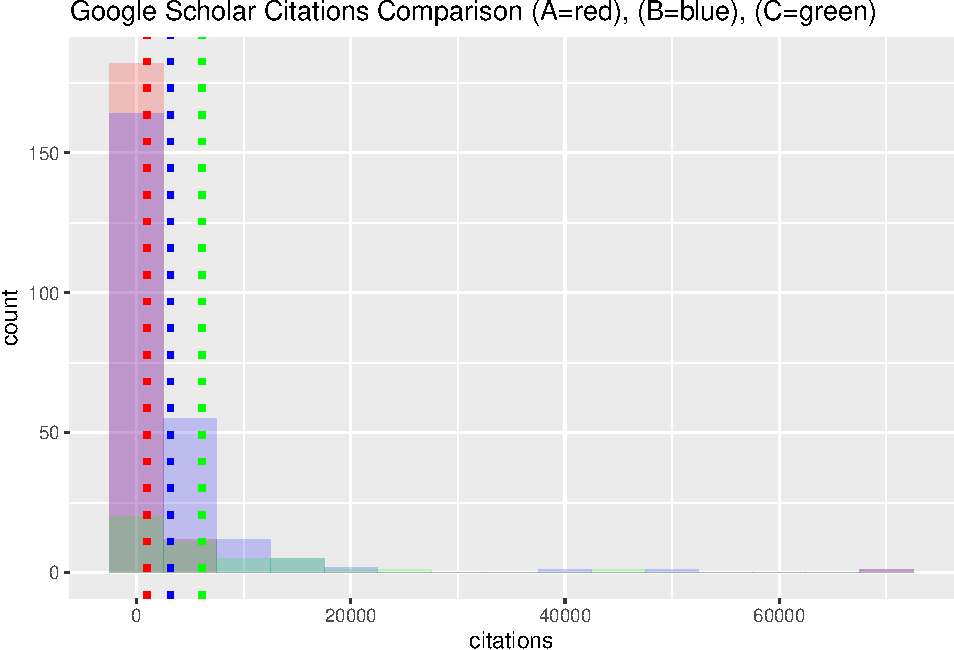
\includegraphics{final_files/figure-latex/unnamed-chunk-56-1.pdf}

The mean number of citations for signers of Letter A is 947.73, and the
median is 161. The mean number of citations for signers of Letter B is
3144.062, and the median is 1246. The mean number of citations for
signers of Letter C is 6074, and the median is 3307.

So it seems by directly comparing populations, signers of Letter A had
less citations than their counterparts on B and C, and that signers of B
had less citations than those on C.

Let's validate this using a permutation test.

\begin{Shaded}
\begin{Highlighting}[]
\NormalTok{muA <-}\StringTok{ }\KeywordTok{mean}\NormalTok{(}\KeywordTok{filter}\NormalTok{(df, (lettergroup }\OperatorTok{==}\StringTok{ "A Only"}\OperatorTok{|}\NormalTok{lettergroup }\OperatorTok{==}\StringTok{ "A and B"}\NormalTok{))}\OperatorTok{$}\NormalTok{citations, }\DataTypeTok{na.rm =} \OtherTok{TRUE}\NormalTok{)}
\NormalTok{muB <-}\StringTok{ }\KeywordTok{mean}\NormalTok{(}\KeywordTok{filter}\NormalTok{(df, (lettergroup }\OperatorTok{==}\StringTok{ "B Only"}\OperatorTok{|}\NormalTok{lettergroup }\OperatorTok{==}\StringTok{ "A and B"}\NormalTok{))}\OperatorTok{$}\NormalTok{citations, }\DataTypeTok{na.rm =} \OtherTok{TRUE}\NormalTok{)}
\NormalTok{muC <-}\StringTok{ }\KeywordTok{mean}\NormalTok{(}\KeywordTok{filter}\NormalTok{(df, (lettergroup }\OperatorTok{==}\StringTok{ "C Only"}\OperatorTok{|}\NormalTok{lettergroup }\OperatorTok{==}\StringTok{ "B and C"}\NormalTok{))}\OperatorTok{$}\NormalTok{citations, }\DataTypeTok{na.rm =} \OtherTok{TRUE}\NormalTok{)}

\NormalTok{val1 <-}\StringTok{ }\NormalTok{muA }\OperatorTok{-}\StringTok{ }\NormalTok{muB}
\NormalTok{val2 <-}\StringTok{ }\NormalTok{muB }\OperatorTok{-}\StringTok{ }\NormalTok{muC}
\NormalTok{val3 <-}\StringTok{ }\NormalTok{muA }\OperatorTok{-}\StringTok{ }\NormalTok{muC}

\KeywordTok{set.seed}\NormalTok{(}\DecValTok{0}\NormalTok{)}
\NormalTok{dist <-}\StringTok{ }\KeywordTok{meanPermutation}\NormalTok{(}\KeywordTok{na.omit}\NormalTok{(df}\OperatorTok{$}\NormalTok{citations),}\DecValTok{10000}\NormalTok{)}

\KeywordTok{hist}\NormalTok{(dist,}
     \DataTypeTok{main =} \StringTok{"Permutation Test on GS citations"}\NormalTok{,}
     \DataTypeTok{xlab =} \StringTok{"Differences in Mean"}\NormalTok{)}
\KeywordTok{abline}\NormalTok{(}\DataTypeTok{v=}\NormalTok{val1, }\DataTypeTok{col =} \StringTok{"red"}\NormalTok{)}
\KeywordTok{abline}\NormalTok{(}\DataTypeTok{v=}\NormalTok{val2, }\DataTypeTok{col =} \StringTok{"blue"}\NormalTok{)}
\KeywordTok{abline}\NormalTok{(}\DataTypeTok{v=}\NormalTok{val3, }\DataTypeTok{col =} \StringTok{"green"}\NormalTok{)}
\end{Highlighting}
\end{Shaded}

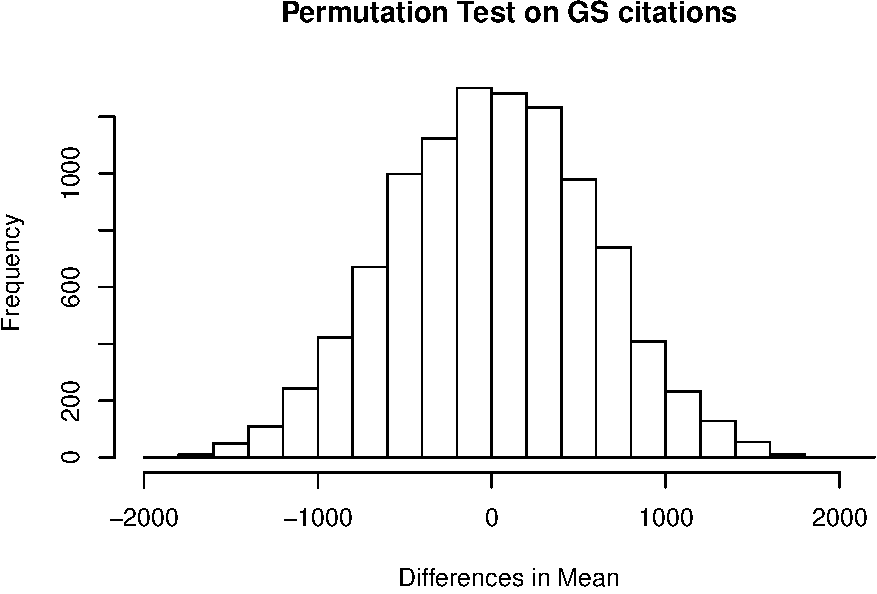
\includegraphics{final_files/figure-latex/unnamed-chunk-58-1.pdf}

All three differences in mean number of citations lie outside of the
induced distribution, so it is unlikely that the observed differences
were due to chance. So we can reject all three null hypotheses, and
deduce that the signers of letter A had less citations than signers of B
and C.

\hypertarget{google-scholar-citations-only-professors}{%
\subsection{Google Scholar Citations Only
Professors}\label{google-scholar-citations-only-professors}}

It is difficult to compare grad students or recently graduates to
professors. So we should subset the data, and reperform the analysis
comparing only professors.

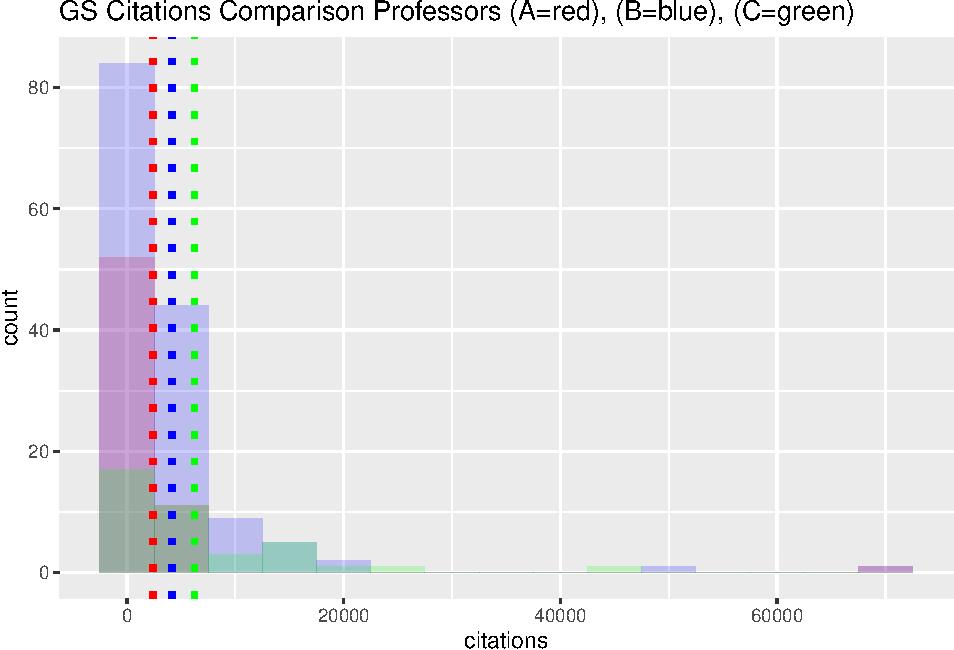
\includegraphics{final_files/figure-latex/unnamed-chunk-59-1.pdf}

The mean number of citations for professors who were signers of Letter A
is 2397.75, and the median is 954. The mean number of citations for
professors who were signers of Letter B is 4136.432, and the median is
1923. The mean number of citations for professors who were signers of
Letter C is 6226.816, and the median is 3307.

So it seems by directly comparing populations, professors on Letter A
had less citations than their counterparts on B and C. Let's validate
this using a permutation test.

\begin{Shaded}
\begin{Highlighting}[]
\NormalTok{muA <-}\StringTok{ }\KeywordTok{mean}\NormalTok{(}\KeywordTok{filter}\NormalTok{(df, ((lettergroup }\OperatorTok{==}\StringTok{ "A Only"}\OperatorTok{|}\NormalTok{lettergroup }\OperatorTok{==}\StringTok{ "A and B"}\NormalTok{)}\OperatorTok{&}\NormalTok{(role}\OperatorTok{==}\StringTok{"professor"}\NormalTok{)))}\OperatorTok{$}\NormalTok{citations, }\DataTypeTok{na.rm =} \OtherTok{TRUE}\NormalTok{)}
\NormalTok{muB <-}\StringTok{ }\KeywordTok{mean}\NormalTok{(}\KeywordTok{filter}\NormalTok{(df, ((lettergroup }\OperatorTok{==}\StringTok{ "B Only"}\OperatorTok{|}\NormalTok{lettergroup }\OperatorTok{==}\StringTok{ "A and B"}\NormalTok{)}\OperatorTok{&}\NormalTok{(role}\OperatorTok{==}\StringTok{"professor"}\NormalTok{)))}\OperatorTok{$}\NormalTok{citations, }\DataTypeTok{na.rm =} \OtherTok{TRUE}\NormalTok{)}
\NormalTok{muC <-}\StringTok{ }\KeywordTok{mean}\NormalTok{(}\KeywordTok{filter}\NormalTok{(df, ((lettergroup }\OperatorTok{==}\StringTok{ "C Only"}\OperatorTok{|}\NormalTok{lettergroup }\OperatorTok{==}\StringTok{ "B and C"}\NormalTok{)}\OperatorTok{&}\NormalTok{(role}\OperatorTok{==}\StringTok{"professor"}\NormalTok{)))}\OperatorTok{$}\NormalTok{citations, }\DataTypeTok{na.rm =} \OtherTok{TRUE}\NormalTok{)}

\NormalTok{val1 <-}\StringTok{ }\NormalTok{muA }\OperatorTok{-}\StringTok{ }\NormalTok{muB}
\NormalTok{val2 <-}\StringTok{ }\NormalTok{muB }\OperatorTok{-}\StringTok{ }\NormalTok{muC}
\NormalTok{val3 <-}\StringTok{ }\NormalTok{muA }\OperatorTok{-}\StringTok{ }\NormalTok{muC}

\KeywordTok{set.seed}\NormalTok{(}\DecValTok{0}\NormalTok{)}
\NormalTok{dist <-}\StringTok{ }\KeywordTok{meanPermutation}\NormalTok{(}\KeywordTok{na.omit}\NormalTok{(df}\OperatorTok{$}\NormalTok{citations),}\DecValTok{10000}\NormalTok{)}

\KeywordTok{hist}\NormalTok{(dist,}
     \DataTypeTok{main =} \StringTok{"Permutation Test on GS citations only professors"}\NormalTok{,}
     \DataTypeTok{xlab =} \StringTok{"Differences in Mean"}\NormalTok{)}
\KeywordTok{abline}\NormalTok{(}\DataTypeTok{v=}\NormalTok{val1, }\DataTypeTok{col =} \StringTok{"red"}\NormalTok{)}
\KeywordTok{abline}\NormalTok{(}\DataTypeTok{v=}\NormalTok{val2, }\DataTypeTok{col =} \StringTok{"blue"}\NormalTok{)}
\KeywordTok{abline}\NormalTok{(}\DataTypeTok{v=}\NormalTok{val3, }\DataTypeTok{col =} \StringTok{"green"}\NormalTok{)}
\end{Highlighting}
\end{Shaded}

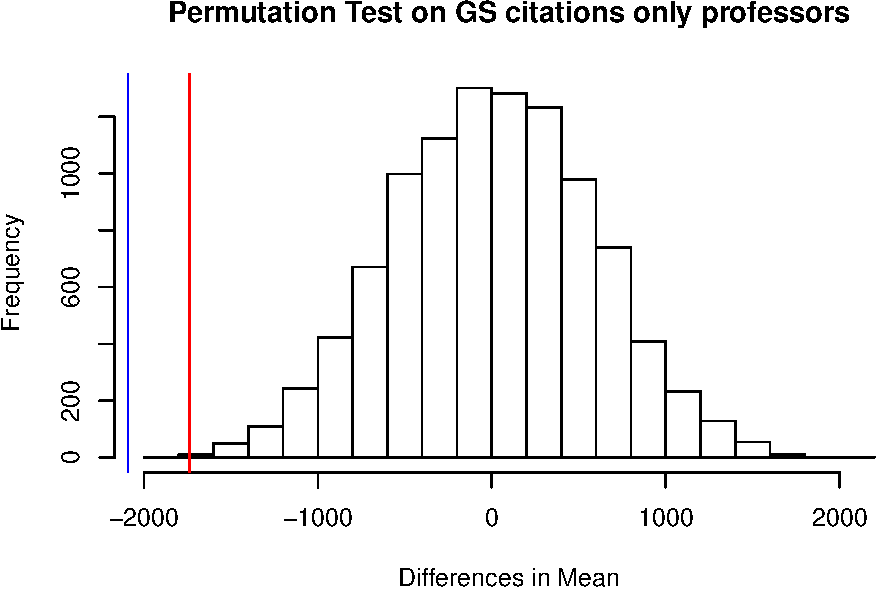
\includegraphics{final_files/figure-latex/unnamed-chunk-61-1.pdf}

The probability that the difference in mean number of citations between
signers, comparing only professors, of A and B is 0.03\%. The difference
between B and C and A and C are both outside the induced distribution.
So it is unlikely that the observed difference in the number of Google
Scholar citations was due to chance, and we may reject all three null
hypotheses.

\hypertarget{google-scholar-citations-per-year}{%
\subsection{Google Scholar Citations per
Year}\label{google-scholar-citations-per-year}}

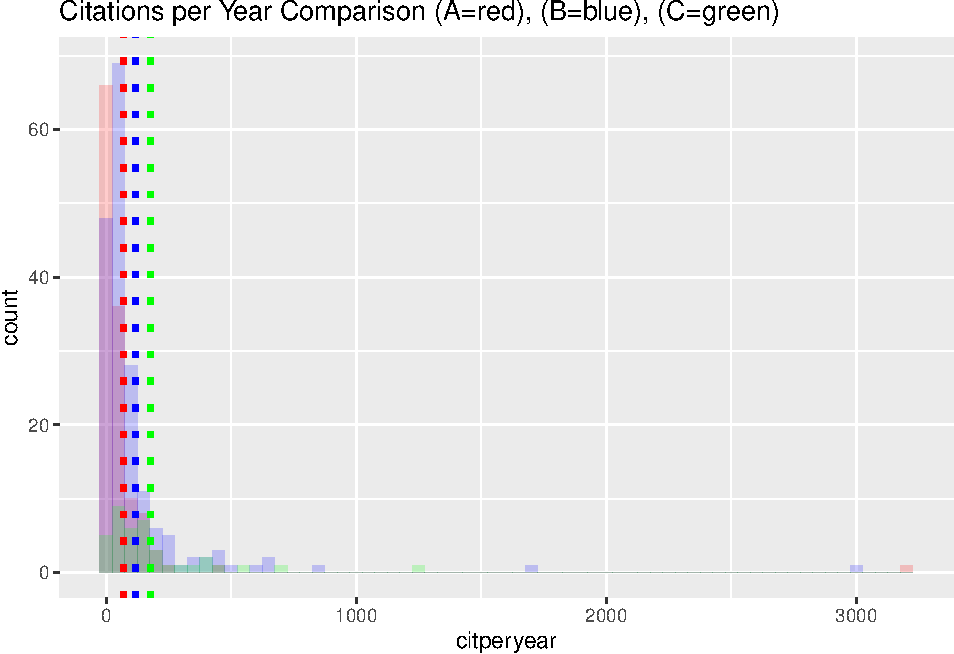
\includegraphics{final_files/figure-latex/unnamed-chunk-63-1.pdf}

The mean number of citations per year for signers of Letter A is 69.25,
and the median is 22.90. The mean number of citations per year for
signers of Letter B is 117.62, and the median is 48.73. The mean number
of citations per year for signers of Letter C is 176.99, and the median
is 116.67.

So it seems by directly comparing populations, professors on Letter A
had less citations per year than their counterparts on B and C. Let's
validate this using a permutation test.

\begin{Shaded}
\begin{Highlighting}[]
\NormalTok{muA <-}\StringTok{ }\KeywordTok{mean}\NormalTok{(}\KeywordTok{filter}\NormalTok{(df, (lettergroup }\OperatorTok{==}\StringTok{ "A Only"}\OperatorTok{|}\NormalTok{lettergroup }\OperatorTok{==}\StringTok{ "A and B"}\NormalTok{))}\OperatorTok{$}\NormalTok{citperyear, }\DataTypeTok{na.rm =} \OtherTok{TRUE}\NormalTok{)}
\NormalTok{muB <-}\StringTok{ }\KeywordTok{mean}\NormalTok{(}\KeywordTok{filter}\NormalTok{(df, (lettergroup }\OperatorTok{==}\StringTok{ "B Only"}\OperatorTok{|}\NormalTok{lettergroup }\OperatorTok{==}\StringTok{ "A and B"}\NormalTok{))}\OperatorTok{$}\NormalTok{citperyear, }\DataTypeTok{na.rm =} \OtherTok{TRUE}\NormalTok{)}
\NormalTok{muC <-}\StringTok{ }\KeywordTok{mean}\NormalTok{(}\KeywordTok{filter}\NormalTok{(df, (lettergroup }\OperatorTok{==}\StringTok{ "C Only"}\OperatorTok{|}\NormalTok{lettergroup }\OperatorTok{==}\StringTok{ "B and C"}\NormalTok{))}\OperatorTok{$}\NormalTok{citperyear, }\DataTypeTok{na.rm =} \OtherTok{TRUE}\NormalTok{)}

\NormalTok{val1 <-}\StringTok{ }\NormalTok{muA }\OperatorTok{-}\StringTok{ }\NormalTok{muB}
\NormalTok{val2 <-}\StringTok{ }\NormalTok{muB }\OperatorTok{-}\StringTok{ }\NormalTok{muC}
\NormalTok{val3 <-}\StringTok{ }\NormalTok{muA }\OperatorTok{-}\StringTok{ }\NormalTok{muC}

\KeywordTok{set.seed}\NormalTok{(}\DecValTok{0}\NormalTok{)}
\NormalTok{dist <-}\StringTok{ }\KeywordTok{meanPermutation}\NormalTok{(}\KeywordTok{na.omit}\NormalTok{(df}\OperatorTok{$}\NormalTok{citperyear),}\DecValTok{10000}\NormalTok{)}

\KeywordTok{hist}\NormalTok{(dist,}
     \DataTypeTok{main =} \StringTok{"Citations per Year Google Scholar"}\NormalTok{,}
     \DataTypeTok{xlab =} \StringTok{"Differences in Mean"}\NormalTok{)}
\KeywordTok{abline}\NormalTok{(}\DataTypeTok{v=}\NormalTok{val1, }\DataTypeTok{col =} \StringTok{"red"}\NormalTok{)}
\KeywordTok{abline}\NormalTok{(}\DataTypeTok{v=}\NormalTok{val2, }\DataTypeTok{col =} \StringTok{"blue"}\NormalTok{)}
\KeywordTok{abline}\NormalTok{(}\DataTypeTok{v=}\NormalTok{val3, }\DataTypeTok{col =} \StringTok{"green"}\NormalTok{)}
\end{Highlighting}
\end{Shaded}

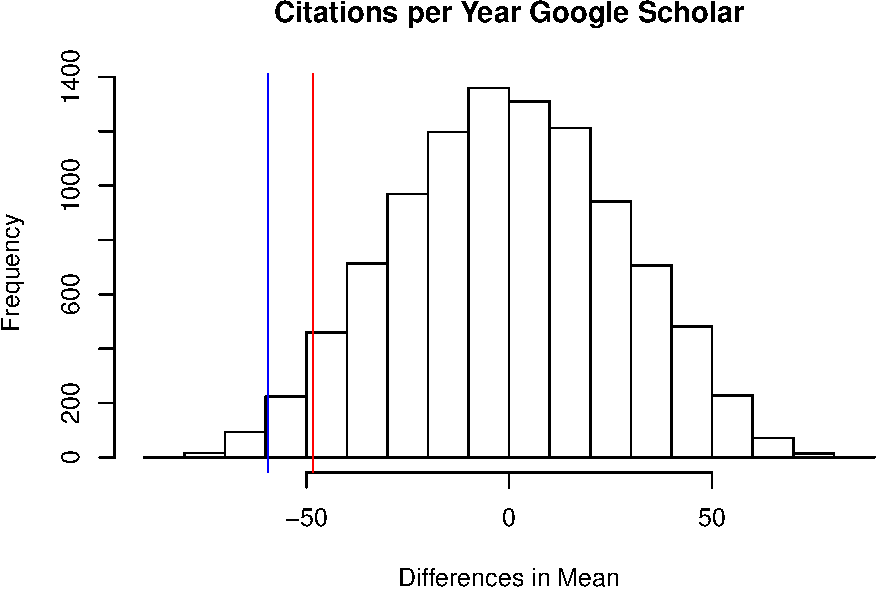
\includegraphics{final_files/figure-latex/unnamed-chunk-65-1.pdf}

The percentage of the induced distribution that is more extreme than the
observed difference in mean number of citations per year between A and B
is 4\%. The percentage of the induced distribution that is more extreme
than the observed difference in mean number of citations per year
between B and C is 1.22\%.The observed difference in mean between A and
C is outside the induced distribution. So it is unlikely that the
observed difference in the number of Google Scholar citations was due to
chance, and we may reject all three null hypotheses.

\hypertarget{google-scholar-citations-per-year-only-professors}{%
\subsection{Google Scholar Citations per Year only
professors}\label{google-scholar-citations-per-year-only-professors}}

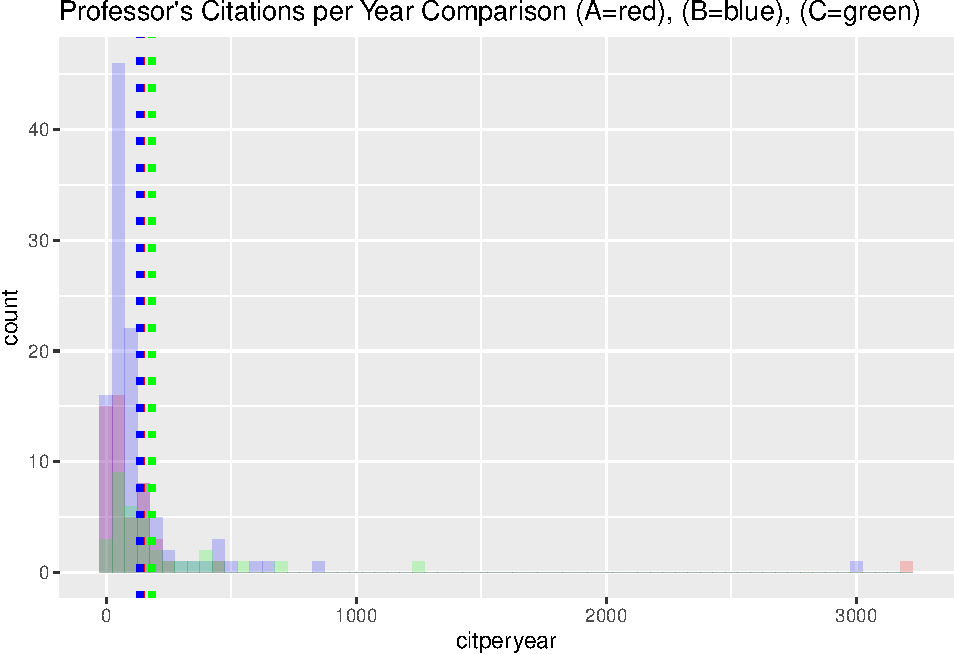
\includegraphics{final_files/figure-latex/unnamed-chunk-67-1.pdf}

The mean number of citations per year for professors who were signers of
Letter A is 139.26, and the median is 47.56. The mean number of
citations per year for professors who were signers of Letter B is
136.14, and the median is 62.81. The mean number of citations per year
for professors who were signers of Letter C is 182.78, and the median is
111.73.

So it seems by directly comparing populations, signers of Letter A had
more citations than their counterparts on B, though less than their
counterparts C.

Let's validate this using a permutation test.

\begin{Shaded}
\begin{Highlighting}[]
\NormalTok{muA <-}\StringTok{ }\KeywordTok{mean}\NormalTok{(}\KeywordTok{filter}\NormalTok{(df, ((lettergroup }\OperatorTok{==}\StringTok{ "A Only"}\OperatorTok{|}\NormalTok{lettergroup }\OperatorTok{==}\StringTok{ "A and B"}\NormalTok{)}\OperatorTok{&}\NormalTok{(role}\OperatorTok{==}\StringTok{"professor"}\NormalTok{)))}\OperatorTok{$}\NormalTok{citperyear, }\DataTypeTok{na.rm =} \OtherTok{TRUE}\NormalTok{)}
\NormalTok{muB <-}\StringTok{ }\KeywordTok{mean}\NormalTok{(}\KeywordTok{filter}\NormalTok{(df, ((lettergroup }\OperatorTok{==}\StringTok{ "B Only"}\OperatorTok{|}\NormalTok{lettergroup }\OperatorTok{==}\StringTok{ "A and B"}\NormalTok{)}\OperatorTok{&}\NormalTok{(role}\OperatorTok{==}\StringTok{"professor"}\NormalTok{)))}\OperatorTok{$}\NormalTok{citperyear, }\DataTypeTok{na.rm =} \OtherTok{TRUE}\NormalTok{)}
\NormalTok{muC <-}\StringTok{ }\KeywordTok{mean}\NormalTok{(}\KeywordTok{filter}\NormalTok{(df, ((lettergroup }\OperatorTok{==}\StringTok{ "C Only"}\OperatorTok{|}\NormalTok{lettergroup }\OperatorTok{==}\StringTok{ "B and C"}\NormalTok{)}\OperatorTok{&}\NormalTok{(role}\OperatorTok{==}\StringTok{"professor"}\NormalTok{)))}\OperatorTok{$}\NormalTok{citperyear, }\DataTypeTok{na.rm =} \OtherTok{TRUE}\NormalTok{)}

\NormalTok{val1 <-}\StringTok{ }\NormalTok{muA }\OperatorTok{-}\StringTok{ }\NormalTok{muB}
\NormalTok{val2 <-}\StringTok{ }\NormalTok{muB }\OperatorTok{-}\StringTok{ }\NormalTok{muC}
\NormalTok{val3 <-}\StringTok{ }\NormalTok{muA }\OperatorTok{-}\StringTok{ }\NormalTok{muC}

\KeywordTok{set.seed}\NormalTok{(}\DecValTok{0}\NormalTok{)}
\NormalTok{dist <-}\StringTok{ }\KeywordTok{meanPermutation}\NormalTok{(}\KeywordTok{na.omit}\NormalTok{(df}\OperatorTok{$}\NormalTok{citperyear),}\DecValTok{10000}\NormalTok{)}

\KeywordTok{hist}\NormalTok{(dist,}
     \DataTypeTok{main =} \StringTok{"GS citations per year Professors Only"}\NormalTok{,}
     \DataTypeTok{xlab =} \StringTok{"Differences in Mean"}\NormalTok{)}
\KeywordTok{abline}\NormalTok{(}\DataTypeTok{v=}\NormalTok{val1, }\DataTypeTok{col =} \StringTok{"red"}\NormalTok{)}
\KeywordTok{abline}\NormalTok{(}\DataTypeTok{v=}\NormalTok{val2, }\DataTypeTok{col =} \StringTok{"blue"}\NormalTok{)}
\KeywordTok{abline}\NormalTok{(}\DataTypeTok{v=}\NormalTok{val3, }\DataTypeTok{col =} \StringTok{"green"}\NormalTok{)}
\end{Highlighting}
\end{Shaded}

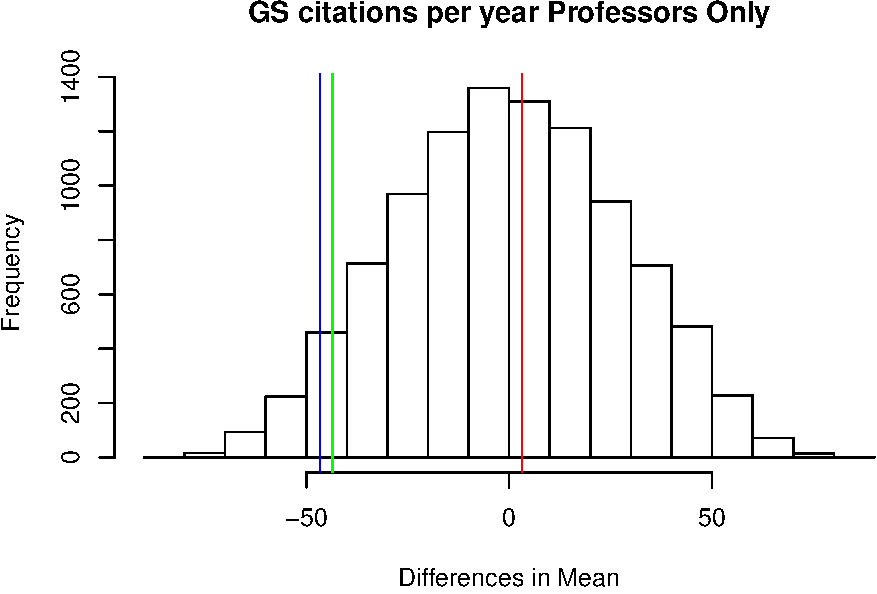
\includegraphics{final_files/figure-latex/unnamed-chunk-69-1.pdf}

About 54.72\% of the induced distribution is more extreme (less) than
the observed difference between A and B, so it is highly likely the
observed difference was due to chance. We fail to reject the null
hypothesis that mean of A is equal to B. Only 4.61\% of the induced
distribution was more extreme than the difference between B and C, and
6.06\% between A and C, so it is unlikely those were due to chance. We
can thus reject the null hypothesis that \(\mu(B)=\mu(C)\) and
\(\mu(C)=\mu(A)\), but with less certainty than the observed difference
for age.

\hypertarget{google-scholar-citations-per-year---female-professors-only}{%
\subsection{Google Scholar Citations Per Year - Female Professors
Only}\label{google-scholar-citations-per-year---female-professors-only}}

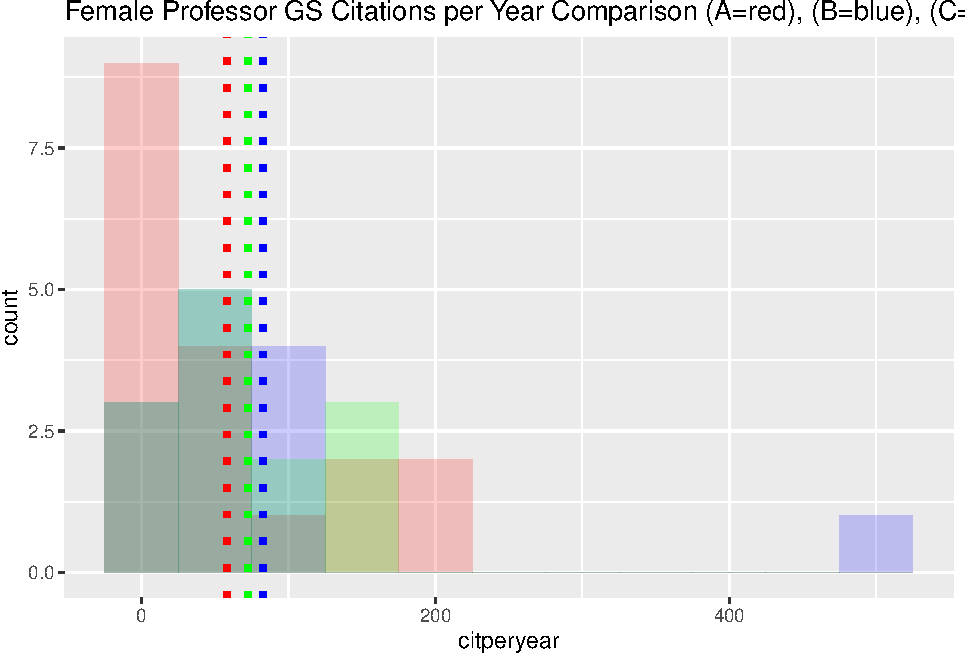
\includegraphics{final_files/figure-latex/unnamed-chunk-71-1.pdf}

The mean number of citations per year for female professors who were
signers of Letter A is 58.25, and the median is 24.28. The mean number
of citations per year for female professors who were signers of Letter B
is 82.40, and the median is 31.94. The mean number of citations per year
for female professors who were signers of Letter C is 72.29, and the
median is 64.56.

So it seems when comparing only female professors, signers of Letter A
had less citations per year than their counterparts on B and C, while
signers of B had more citations per year than C.

Let's validate this using a permutation test.

\begin{Shaded}
\begin{Highlighting}[]
\NormalTok{muA <-}\StringTok{ }\KeywordTok{mean}\NormalTok{(}\KeywordTok{filter}\NormalTok{(df, ((lettergroup }\OperatorTok{==}\StringTok{ "A Only"}\OperatorTok{|}\NormalTok{lettergroup }\OperatorTok{==}\StringTok{ "A and B"}\NormalTok{)}\OperatorTok{&}\NormalTok{(role}\OperatorTok{==}\StringTok{"professor"}\NormalTok{)}\OperatorTok{&}\NormalTok{(gender}\OperatorTok{==}\StringTok{"woman"}\NormalTok{)))}\OperatorTok{$}\NormalTok{citperyear, }\DataTypeTok{na.rm =} \OtherTok{TRUE}\NormalTok{)}
\NormalTok{muB <-}\StringTok{ }\KeywordTok{mean}\NormalTok{(}\KeywordTok{filter}\NormalTok{(df, ((lettergroup }\OperatorTok{==}\StringTok{ "B Only"}\OperatorTok{|}\NormalTok{lettergroup }\OperatorTok{==}\StringTok{ "A and B"}\NormalTok{)}\OperatorTok{&}\NormalTok{(role}\OperatorTok{==}\StringTok{"professor"}\NormalTok{)}\OperatorTok{&}\NormalTok{(gender}\OperatorTok{==}\StringTok{"woman"}\NormalTok{)))}\OperatorTok{$}\NormalTok{citperyear, }\DataTypeTok{na.rm =} \OtherTok{TRUE}\NormalTok{)}
\NormalTok{muC <-}\StringTok{ }\KeywordTok{mean}\NormalTok{(}\KeywordTok{filter}\NormalTok{(df, ((lettergroup }\OperatorTok{==}\StringTok{ "C Only"}\OperatorTok{|}\NormalTok{lettergroup }\OperatorTok{==}\StringTok{ "B and C"}\NormalTok{)}\OperatorTok{&}\NormalTok{(role}\OperatorTok{==}\StringTok{"professor"}\NormalTok{)}\OperatorTok{&}\NormalTok{(gender}\OperatorTok{==}\StringTok{"woman"}\NormalTok{)))}\OperatorTok{$}\NormalTok{citperyear, }\DataTypeTok{na.rm =} \OtherTok{TRUE}\NormalTok{)}

\NormalTok{val1 <-}\StringTok{ }\NormalTok{muA }\OperatorTok{-}\StringTok{ }\NormalTok{muB}
\NormalTok{val2 <-}\StringTok{ }\NormalTok{muB }\OperatorTok{-}\StringTok{ }\NormalTok{muC}
\NormalTok{val3 <-}\StringTok{ }\NormalTok{muA }\OperatorTok{-}\StringTok{ }\NormalTok{muC}

\KeywordTok{set.seed}\NormalTok{(}\DecValTok{0}\NormalTok{)}


\NormalTok{dist <-}\StringTok{ }\KeywordTok{meanPermutation}\NormalTok{(}\KeywordTok{na.omit}\NormalTok{(}\KeywordTok{filter}\NormalTok{(df, ((gender}\OperatorTok{==}\StringTok{"woman"}\NormalTok{)}\OperatorTok{&}\NormalTok{(role}\OperatorTok{==}\StringTok{"professor"}\NormalTok{)))}\OperatorTok{$}\NormalTok{citperyear),}\DecValTok{10000}\NormalTok{)}

\KeywordTok{hist}\NormalTok{(dist,}
     \DataTypeTok{main =} \StringTok{"GS citperyear Female Professors"}\NormalTok{,}
     \DataTypeTok{xlab =} \StringTok{"Differences in Mean"}\NormalTok{)}
\KeywordTok{abline}\NormalTok{(}\DataTypeTok{v=}\NormalTok{val1, }\DataTypeTok{col =} \StringTok{"red"}\NormalTok{)}
\KeywordTok{abline}\NormalTok{(}\DataTypeTok{v=}\NormalTok{val2, }\DataTypeTok{col =} \StringTok{"blue"}\NormalTok{)}
\KeywordTok{abline}\NormalTok{(}\DataTypeTok{v=}\NormalTok{val3, }\DataTypeTok{col =} \StringTok{"green"}\NormalTok{)}
\end{Highlighting}
\end{Shaded}

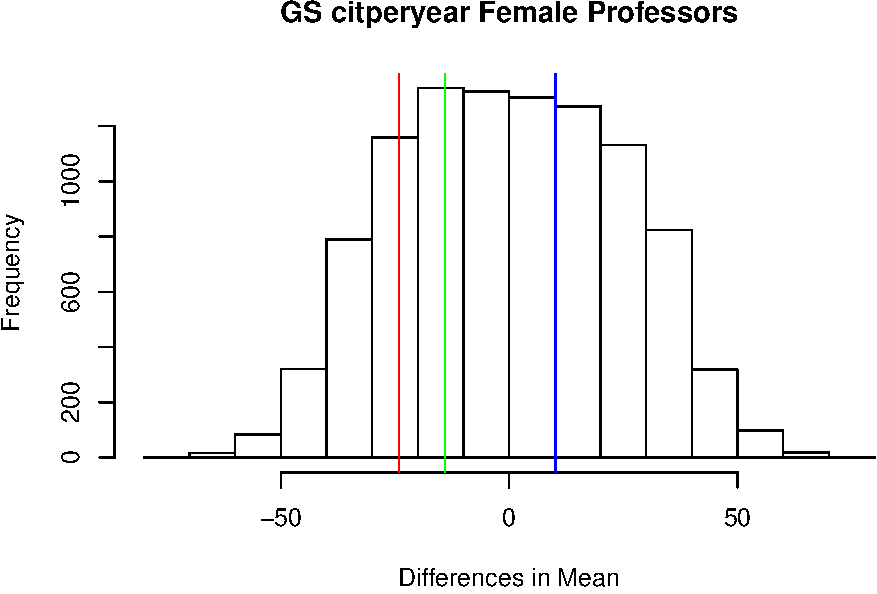
\includegraphics{final_files/figure-latex/unnamed-chunk-73-1.pdf}

18\% of the induced distribution was more extreme than the observed
difference in mean between A and B. 63.52\% of the induced distribution
was more extreme than the observed difference in mean between B and C.
31.56\% of the induced distribution was more extreme than the observed
difference in ean between A and C. So all of these had a high likelihood
of being produced by chance, and we fail to reject all three null
hypotheses.


\end{document}
